% Options for packages loaded elsewhere
\PassOptionsToPackage{unicode}{hyperref}
\PassOptionsToPackage{hyphens}{url}
\PassOptionsToPackage{dvipsnames,svgnames,x11names}{xcolor}
%
\documentclass[
  letterpaper,
  DIV=11,
  numbers=noendperiod,
  titlepage]{scrartcl}

\usepackage{amsmath,amssymb}
\usepackage{iftex}
\ifPDFTeX
  \usepackage[T1]{fontenc}
  \usepackage[utf8]{inputenc}
  \usepackage{textcomp} % provide euro and other symbols
\else % if luatex or xetex
  \usepackage{unicode-math}
  \defaultfontfeatures{Scale=MatchLowercase}
  \defaultfontfeatures[\rmfamily]{Ligatures=TeX,Scale=1}
\fi
\usepackage{lmodern}
\ifPDFTeX\else  
    % xetex/luatex font selection
\fi
% Use upquote if available, for straight quotes in verbatim environments
\IfFileExists{upquote.sty}{\usepackage{upquote}}{}
\IfFileExists{microtype.sty}{% use microtype if available
  \usepackage[]{microtype}
  \UseMicrotypeSet[protrusion]{basicmath} % disable protrusion for tt fonts
}{}
\makeatletter
\@ifundefined{KOMAClassName}{% if non-KOMA class
  \IfFileExists{parskip.sty}{%
    \usepackage{parskip}
  }{% else
    \setlength{\parindent}{0pt}
    \setlength{\parskip}{6pt plus 2pt minus 1pt}}
}{% if KOMA class
  \KOMAoptions{parskip=half}}
\makeatother
\usepackage{xcolor}
\usepackage[top=20mm,bottom=5mm]{geometry}
\setlength{\emergencystretch}{3em} % prevent overfull lines
\setcounter{secnumdepth}{-\maxdimen} % remove section numbering
% Make \paragraph and \subparagraph free-standing
\ifx\paragraph\undefined\else
  \let\oldparagraph\paragraph
  \renewcommand{\paragraph}[1]{\oldparagraph{#1}\mbox{}}
\fi
\ifx\subparagraph\undefined\else
  \let\oldsubparagraph\subparagraph
  \renewcommand{\subparagraph}[1]{\oldsubparagraph{#1}\mbox{}}
\fi


\providecommand{\tightlist}{%
  \setlength{\itemsep}{0pt}\setlength{\parskip}{0pt}}\usepackage{longtable,booktabs,array}
\usepackage{calc} % for calculating minipage widths
% Correct order of tables after \paragraph or \subparagraph
\usepackage{etoolbox}
\makeatletter
\patchcmd\longtable{\par}{\if@noskipsec\mbox{}\fi\par}{}{}
\makeatother
% Allow footnotes in longtable head/foot
\IfFileExists{footnotehyper.sty}{\usepackage{footnotehyper}}{\usepackage{footnote}}
\makesavenoteenv{longtable}
\usepackage{graphicx}
\makeatletter
\def\maxwidth{\ifdim\Gin@nat@width>\linewidth\linewidth\else\Gin@nat@width\fi}
\def\maxheight{\ifdim\Gin@nat@height>\textheight\textheight\else\Gin@nat@height\fi}
\makeatother
% Scale images if necessary, so that they will not overflow the page
% margins by default, and it is still possible to overwrite the defaults
% using explicit options in \includegraphics[width, height, ...]{}
\setkeys{Gin}{width=\maxwidth,height=\maxheight,keepaspectratio}
% Set default figure placement to htbp
\makeatletter
\def\fps@figure{htbp}
\makeatother

\usepackage{booktabs}
\usepackage{longtable}
\usepackage{array}
\usepackage{multirow}
\usepackage{wrapfig}
\usepackage{float}
\usepackage{colortbl}
\usepackage{pdflscape}
\usepackage{tabu}
\usepackage{threeparttable}
\usepackage{threeparttablex}
\usepackage[normalem]{ulem}
\usepackage{makecell}
\usepackage{xcolor}
\usepackage{typearea}
\usepackage{caption}
\captionsetup{font=tiny}
\KOMAoption{captions}{tableheading}
\makeatletter
\makeatother
\makeatletter
\makeatother
\makeatletter
\@ifpackageloaded{caption}{}{\usepackage{caption}}
\AtBeginDocument{%
\ifdefined\contentsname
  \renewcommand*\contentsname{Table of contents}
\else
  \newcommand\contentsname{Table of contents}
\fi
\ifdefined\listfigurename
  \renewcommand*\listfigurename{List of Figures}
\else
  \newcommand\listfigurename{List of Figures}
\fi
\ifdefined\listtablename
  \renewcommand*\listtablename{List of Tables}
\else
  \newcommand\listtablename{List of Tables}
\fi
\ifdefined\figurename
  \renewcommand*\figurename{Figure}
\else
  \newcommand\figurename{Figure}
\fi
\ifdefined\tablename
  \renewcommand*\tablename{Table}
\else
  \newcommand\tablename{Table}
\fi
}
\@ifpackageloaded{float}{}{\usepackage{float}}
\floatstyle{ruled}
\@ifundefined{c@chapter}{\newfloat{codelisting}{h}{lop}}{\newfloat{codelisting}{h}{lop}[chapter]}
\floatname{codelisting}{Listing}
\newcommand*\listoflistings{\listof{codelisting}{List of Listings}}
\makeatother
\makeatletter
\@ifpackageloaded{caption}{}{\usepackage{caption}}
\@ifpackageloaded{subcaption}{}{\usepackage{subcaption}}
\makeatother
\makeatletter
\@ifpackageloaded{tcolorbox}{}{\usepackage[skins,breakable]{tcolorbox}}
\makeatother
\makeatletter
\@ifundefined{shadecolor}{\definecolor{shadecolor}{rgb}{.97, .97, .97}}
\makeatother
\makeatletter
\makeatother
\makeatletter
\makeatother
\ifLuaTeX
  \usepackage{selnolig}  % disable illegal ligatures
\fi
\IfFileExists{bookmark.sty}{\usepackage{bookmark}}{\usepackage{hyperref}}
\IfFileExists{xurl.sty}{\usepackage{xurl}}{} % add URL line breaks if available
\urlstyle{same} % disable monospaced font for URLs
\hypersetup{
  pdftitle={Simulation Result For Two-Level Intercept Model With High Prevalence},
  pdfauthor={Shafayet Khan Shafee},
  colorlinks=true,
  linkcolor={blue},
  filecolor={Maroon},
  citecolor={Blue},
  urlcolor={Blue},
  pdfcreator={LaTeX via pandoc}}

\title{Simulation Result For Two-Level Intercept Model With High
Prevalence}
\usepackage{etoolbox}
\makeatletter
\providecommand{\subtitle}[1]
\author{Shafayet Khan Shafee}
\date{03 September 2023}

\begin{document}
\maketitle
\ifdefined\Shaded\renewenvironment{Shaded}{\begin{tcolorbox}[enhanced, interior hidden, frame hidden, sharp corners, breakable, boxrule=0pt, borderline west={3pt}{0pt}{shadecolor}]}{\end{tcolorbox}}\fi

\newpage

\hypertarget{histograms-for-logwidehatmor}{%
\section{\texorpdfstring{Histograms for
\(log(\widehat{MOR})\)}{Histograms for log(\textbackslash widehat\{MOR\})}}\label{histograms-for-logwidehatmor}}

\vspace{10mm}

\begin{figure}

\begin{minipage}[t]{0.05\linewidth}

{\centering 

\rotatebox[origin=br]{90}{\tiny Cluster Number 10}

}

\end{minipage}%
%
\begin{minipage}[t]{0.24\linewidth}

{\centering 

\raisebox{-\height}{

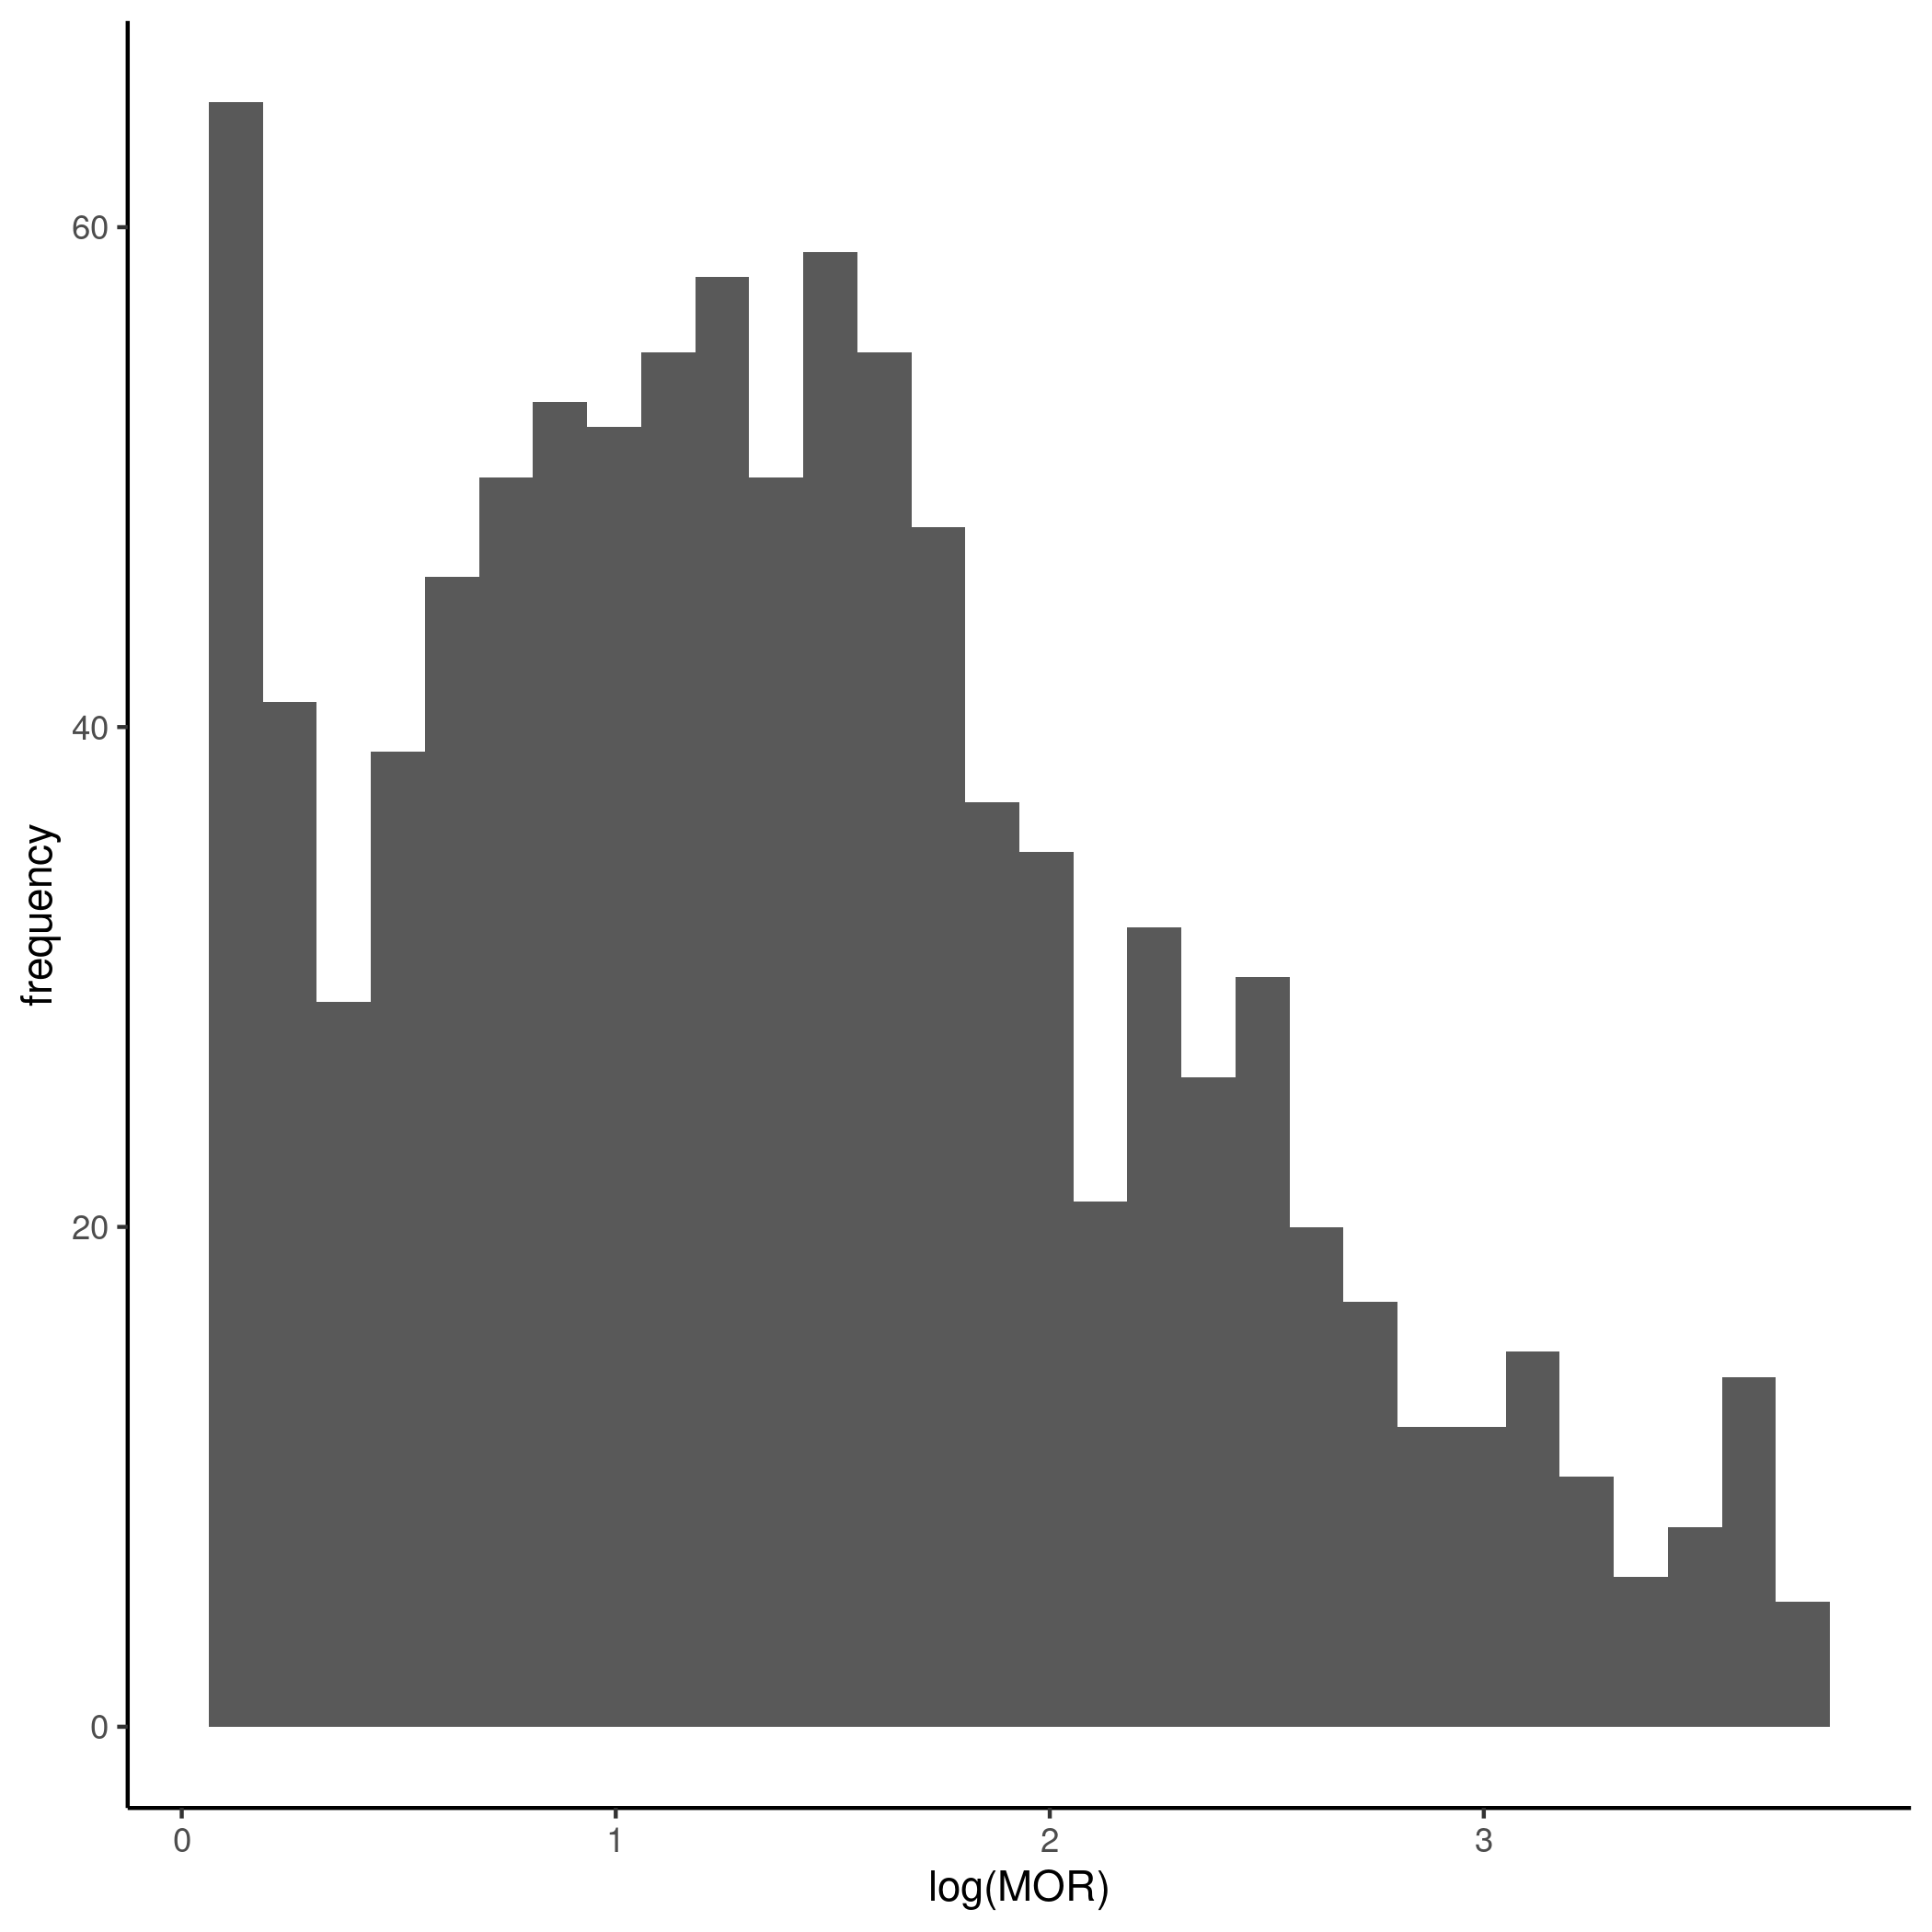
\includegraphics{../../plots/two-lvl-ran-int/high-prev/hist_10_5_two_lvl_high_prev.png}

}

\caption{Cluster size 5}

}

\end{minipage}%
%
\begin{minipage}[t]{0.24\linewidth}

{\centering 

\raisebox{-\height}{

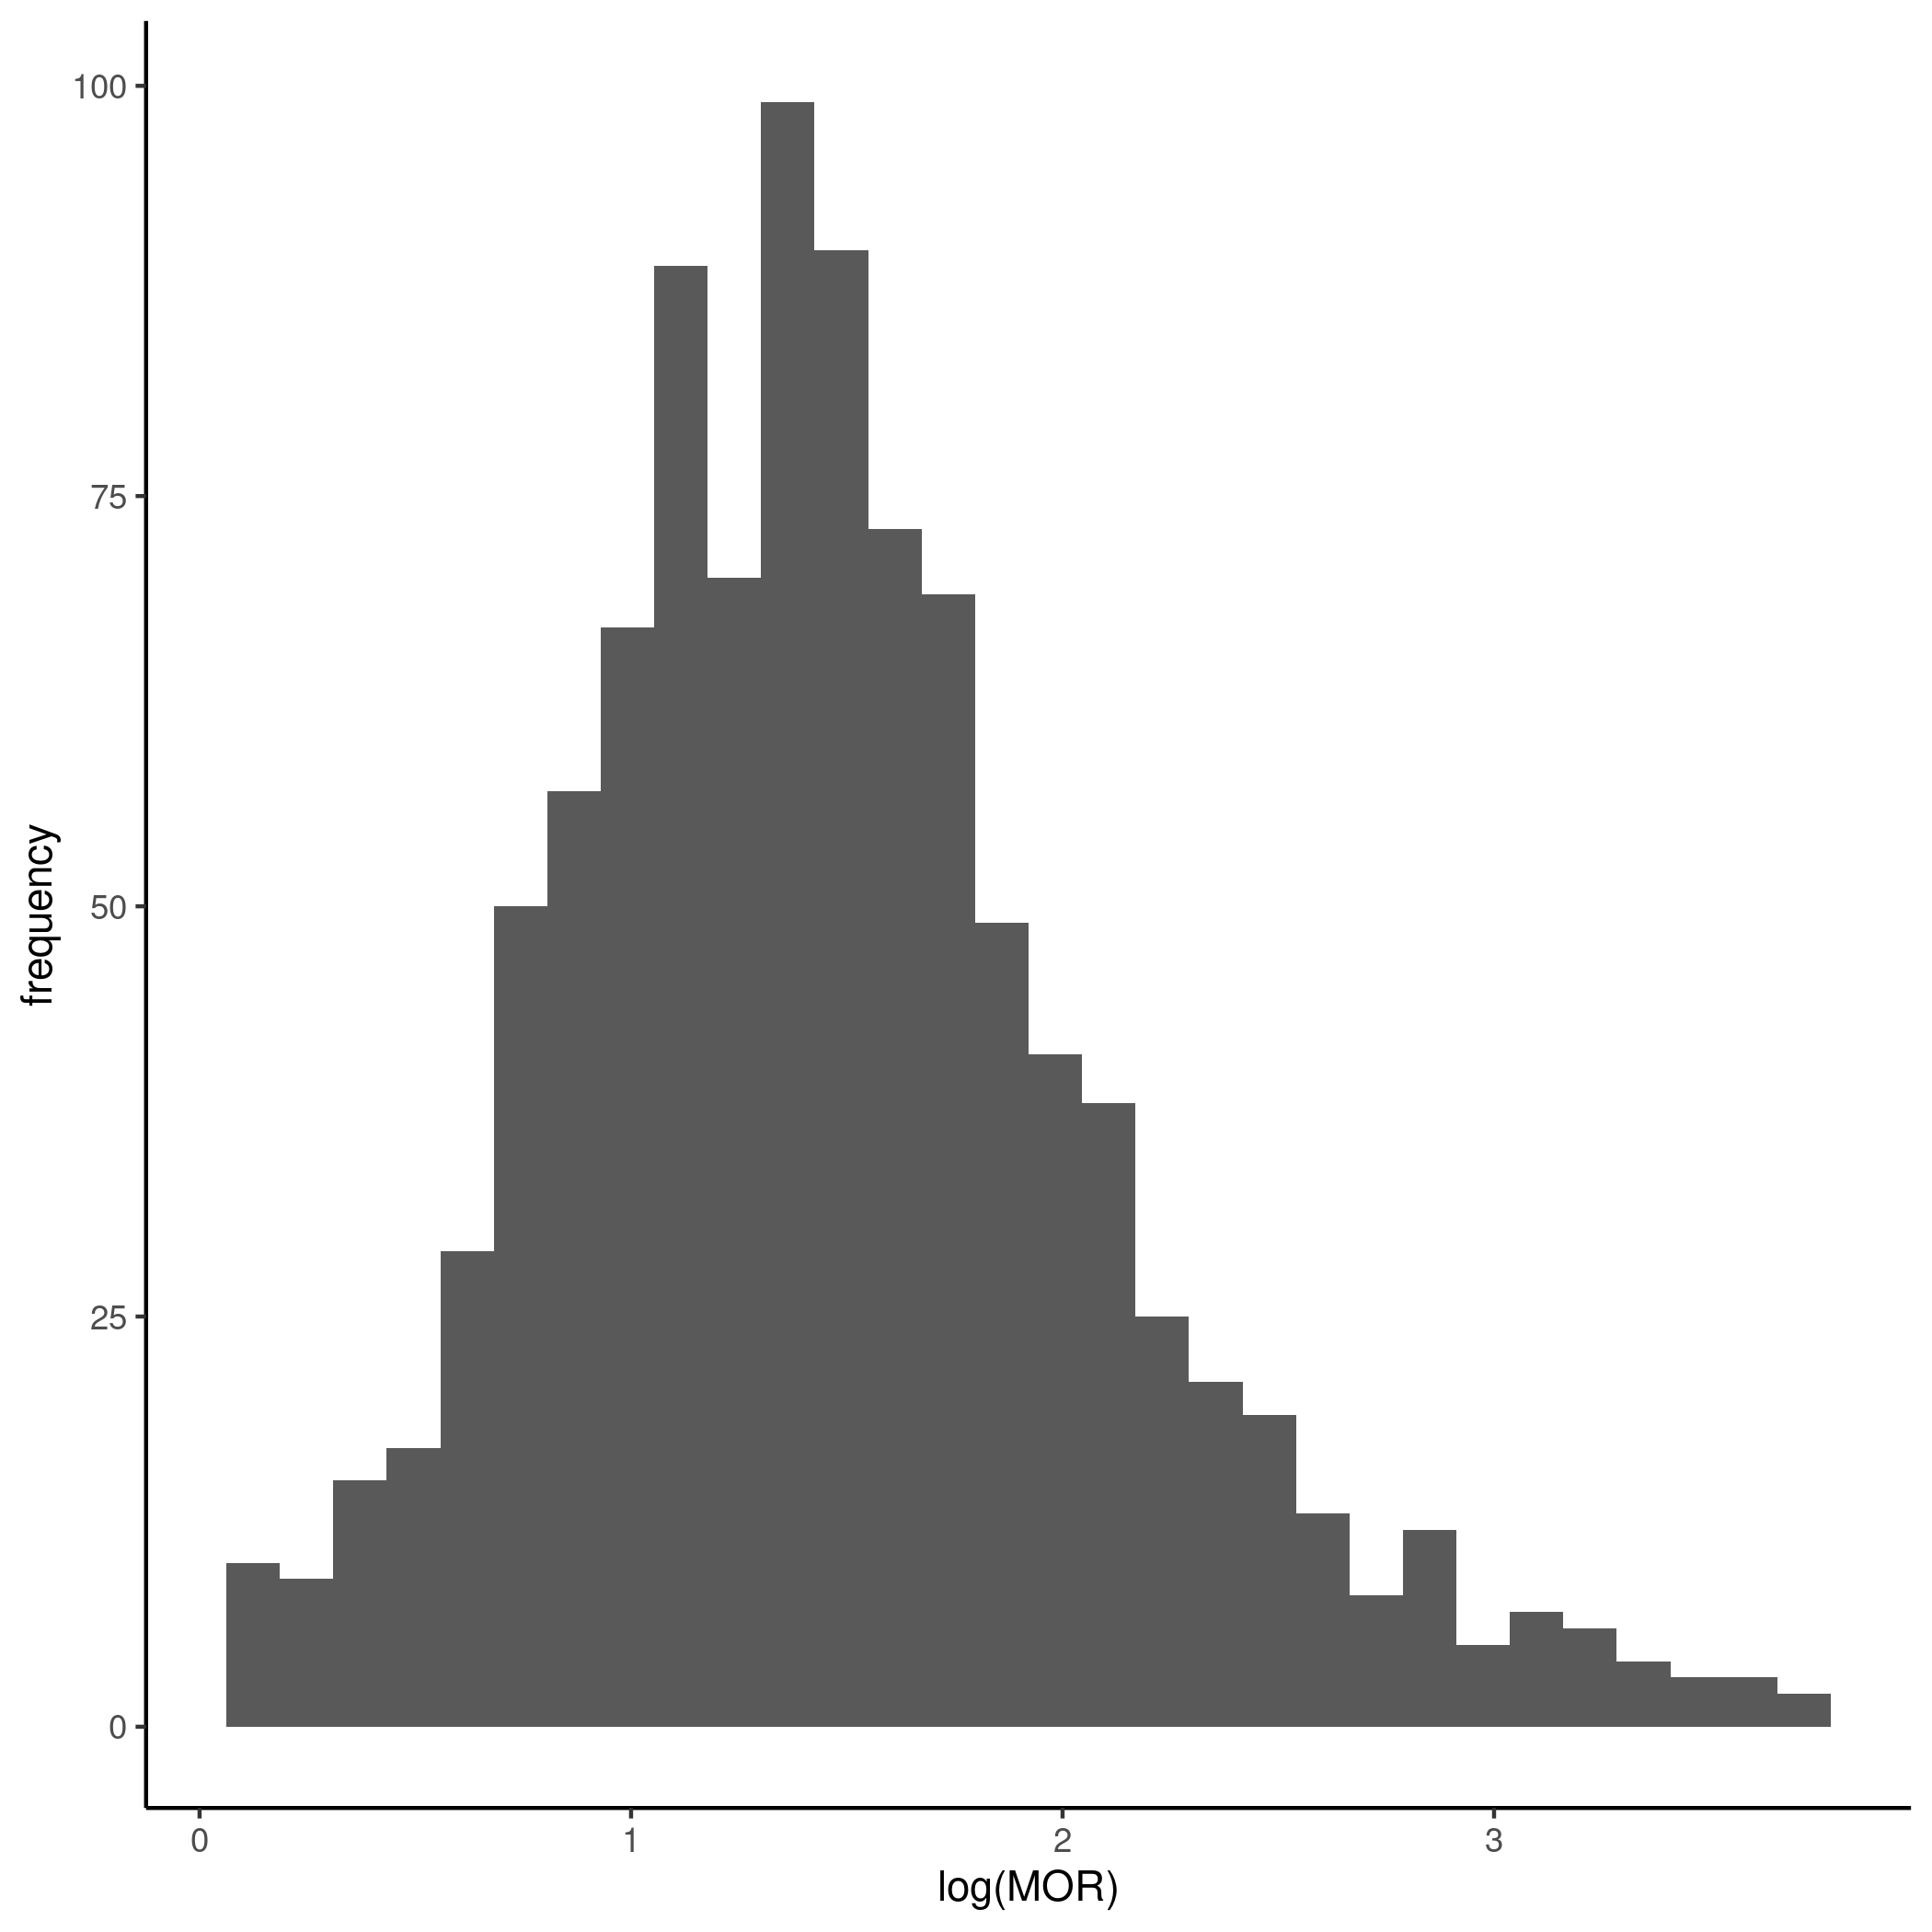
\includegraphics{../../plots/two-lvl-ran-int/high-prev/hist_10_10_two_lvl_high_prev.png}

}

\caption{Cluster size 10}

}

\end{minipage}%
%
\begin{minipage}[t]{0.24\linewidth}

{\centering 

\raisebox{-\height}{

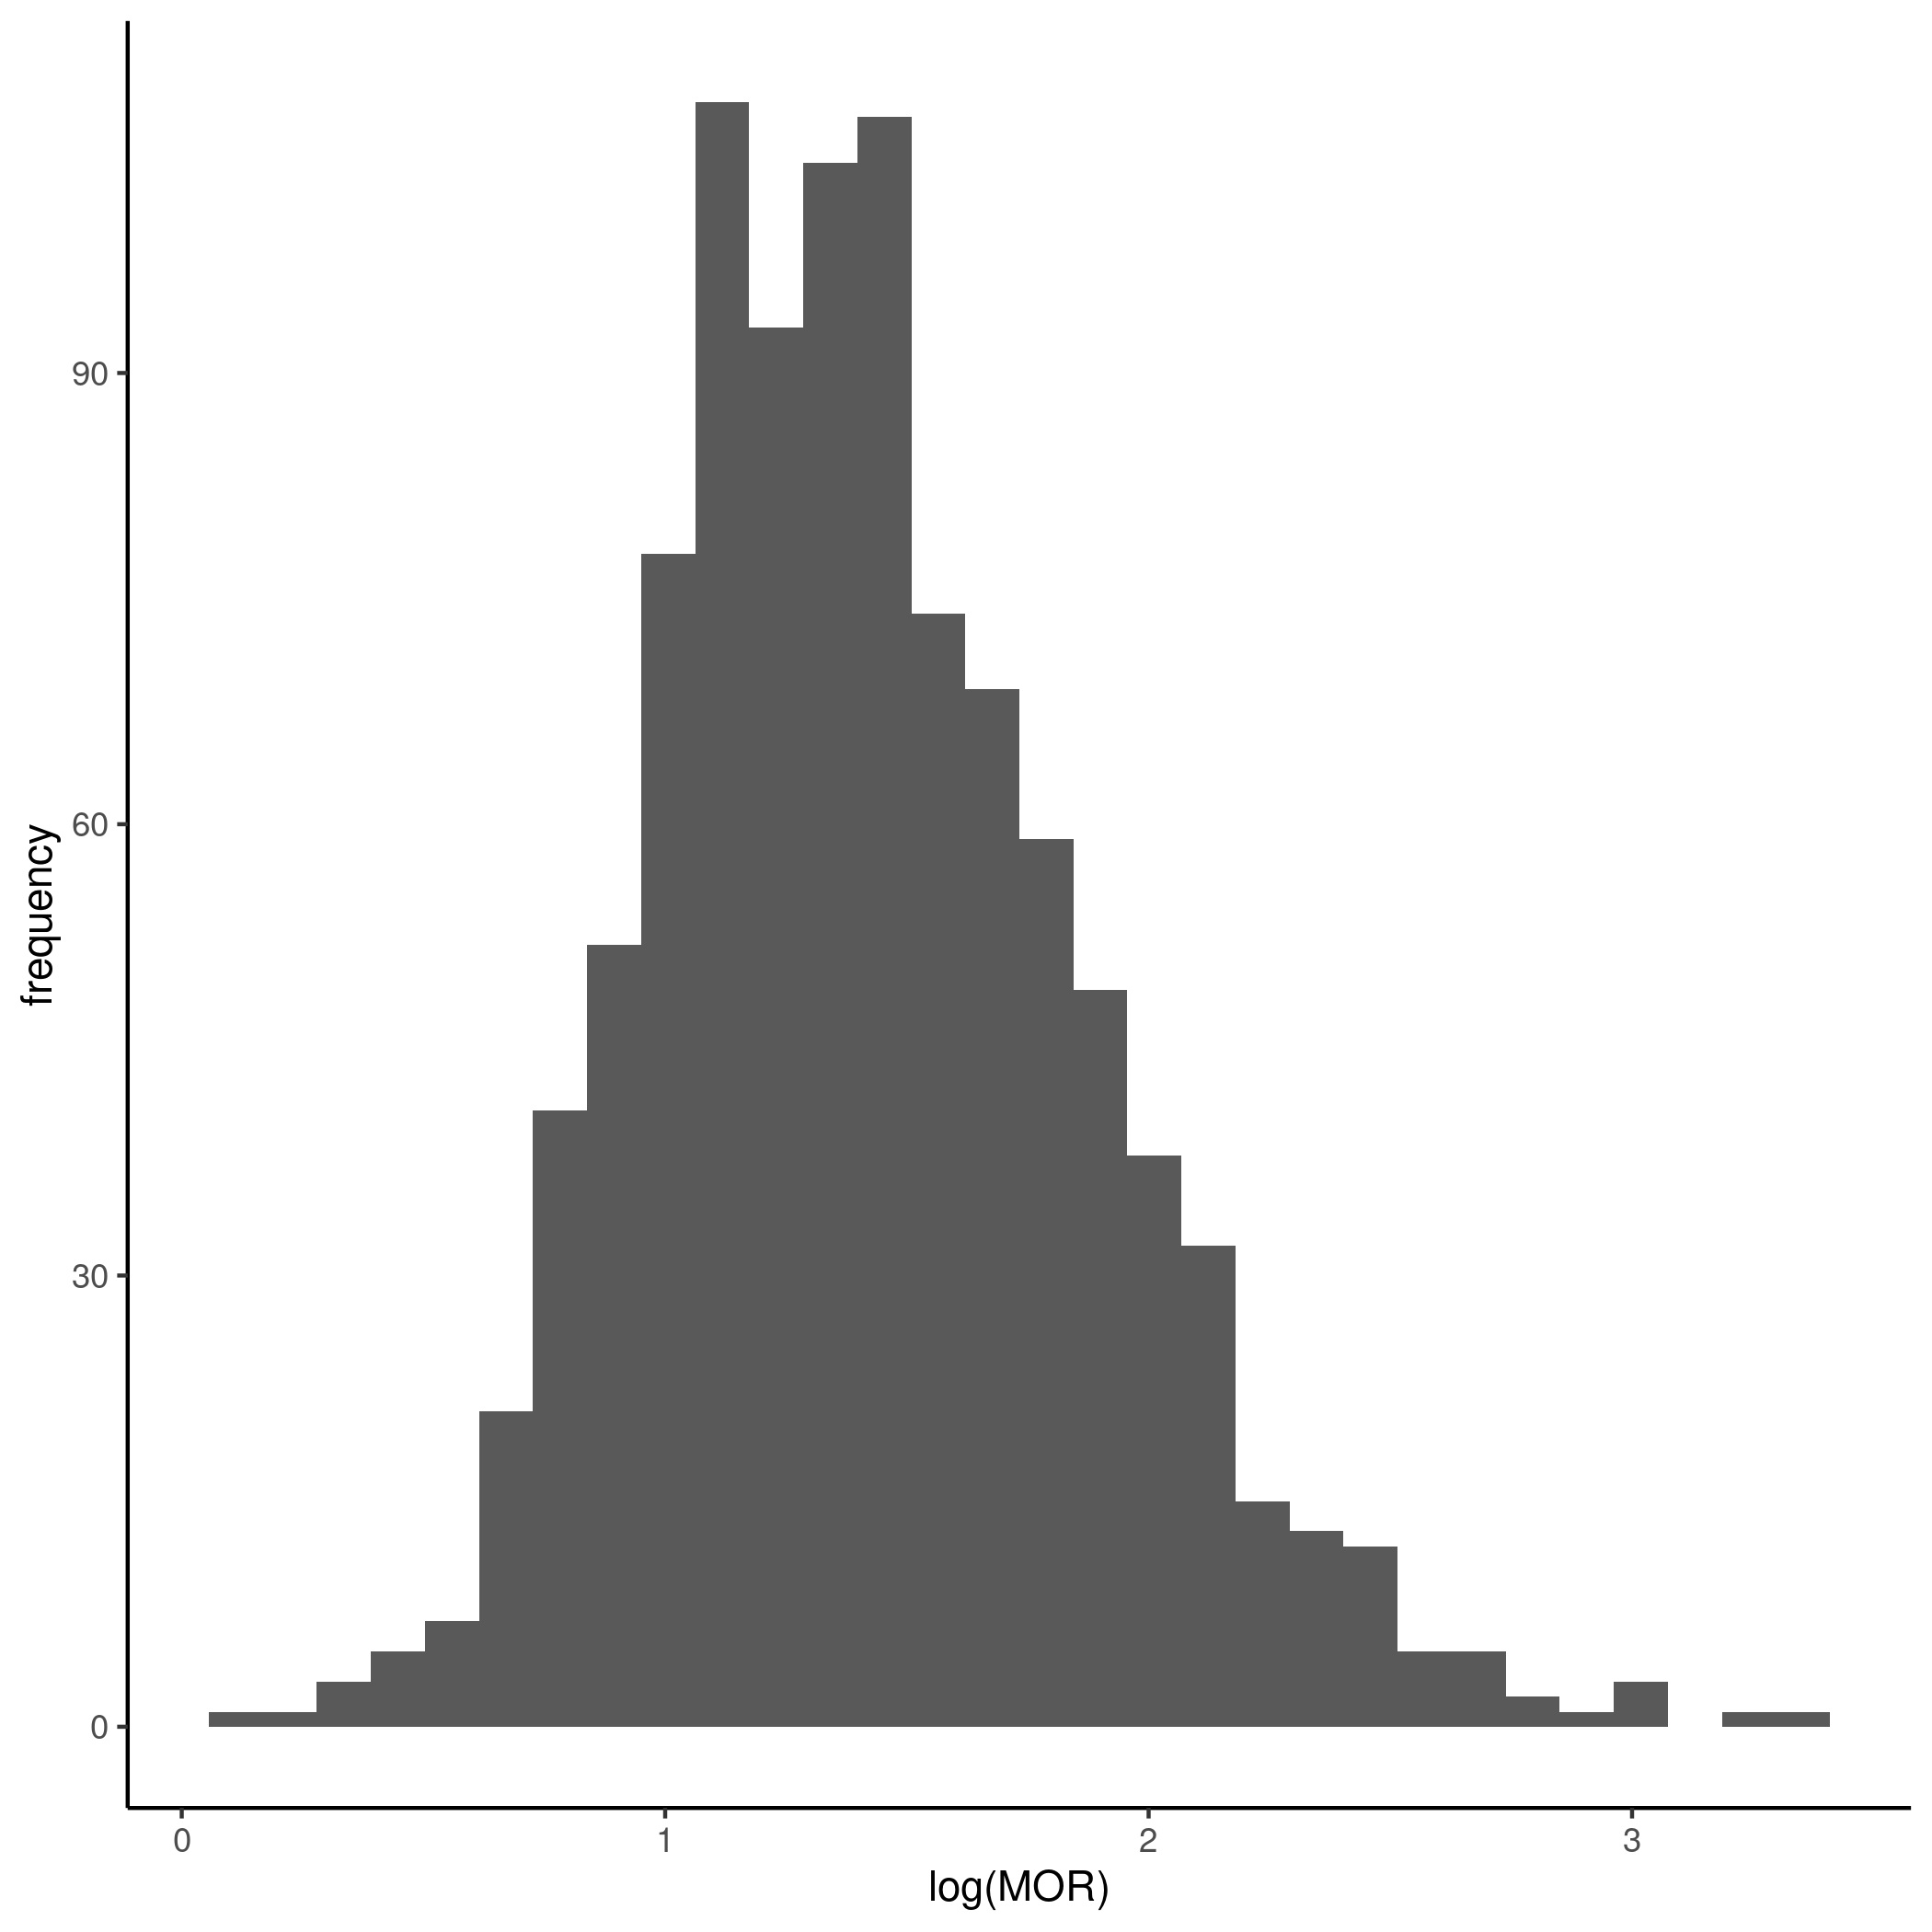
\includegraphics{../../plots/two-lvl-ran-int/high-prev/hist_10_30_two_lvl_high_prev.png}

}

\caption{Cluster size 30}

}

\end{minipage}%
%
\begin{minipage}[t]{0.24\linewidth}

{\centering 

\raisebox{-\height}{

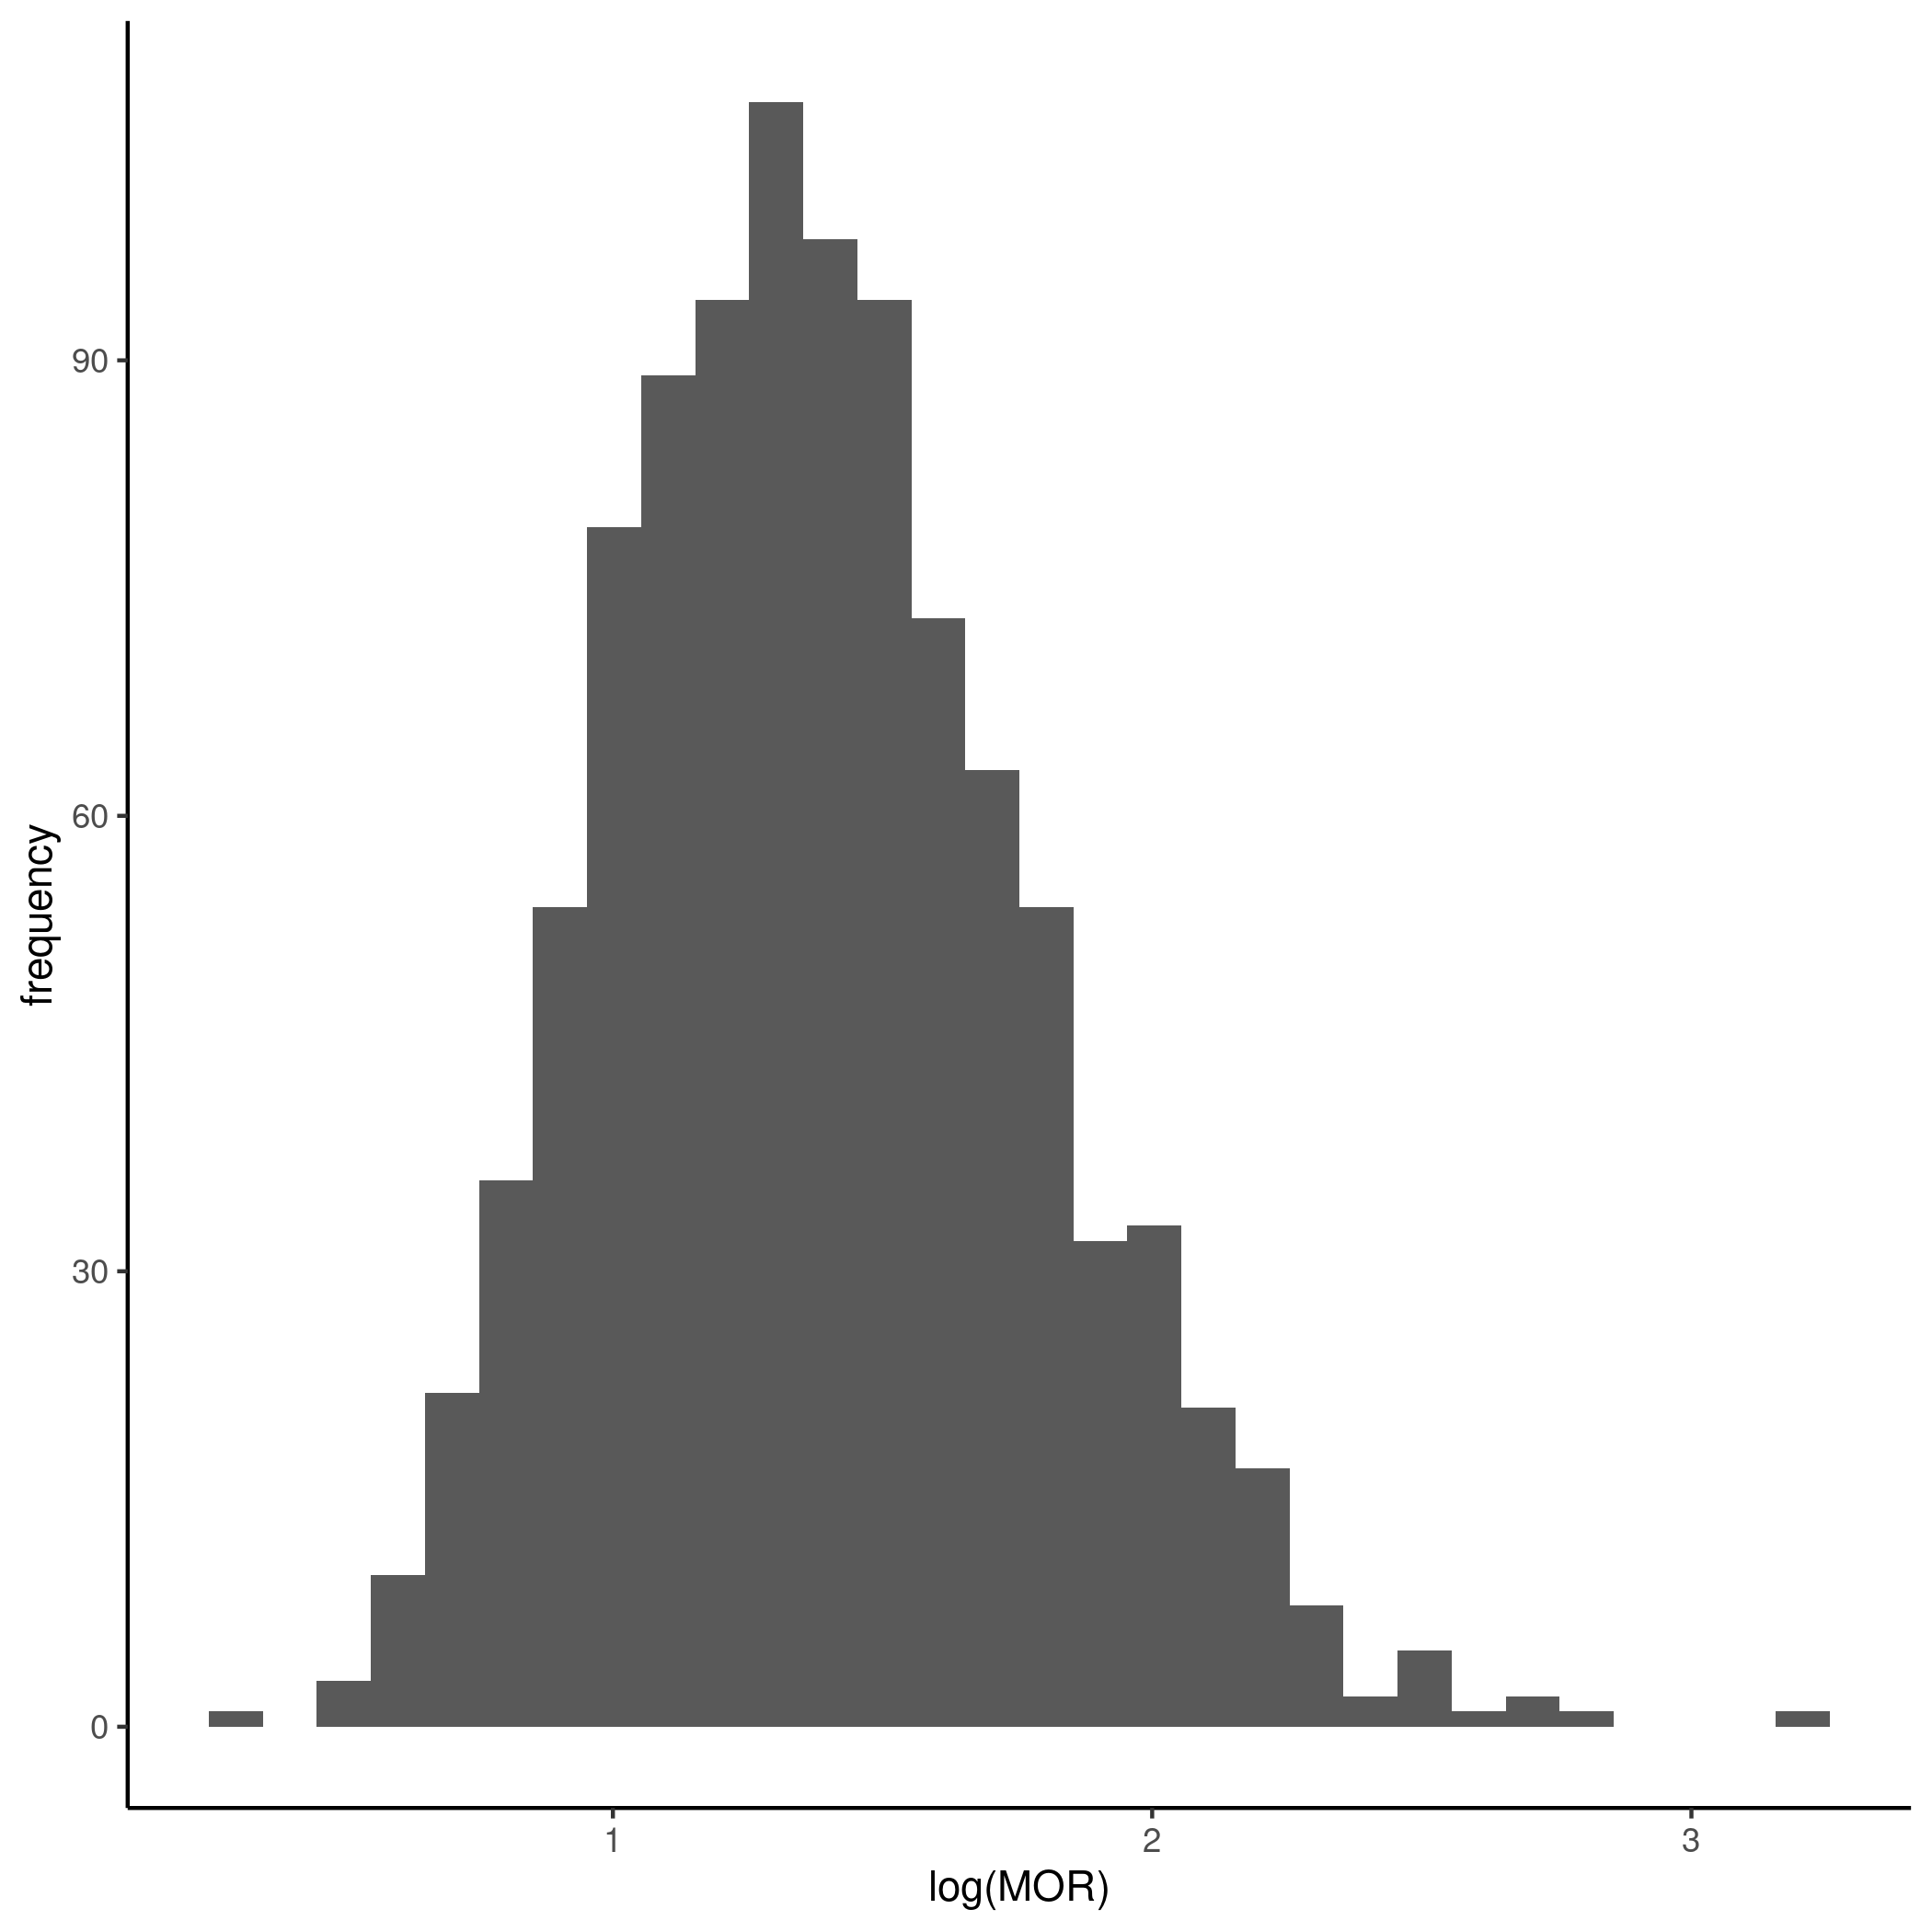
\includegraphics{../../plots/two-lvl-ran-int/high-prev/hist_10_50_two_lvl_high_prev.png}

}

\caption{Cluster size 50}

}

\end{minipage}%
\newline
\begin{minipage}[t]{\linewidth}

{\centering 

~

}

\end{minipage}%
\newline
\begin{minipage}[t]{0.05\linewidth}

{\centering 

\rotatebox[origin=br]{90}{\tiny Cluster Number 30}

}

\end{minipage}%
%
\begin{minipage}[t]{0.24\linewidth}

{\centering 

\raisebox{-\height}{

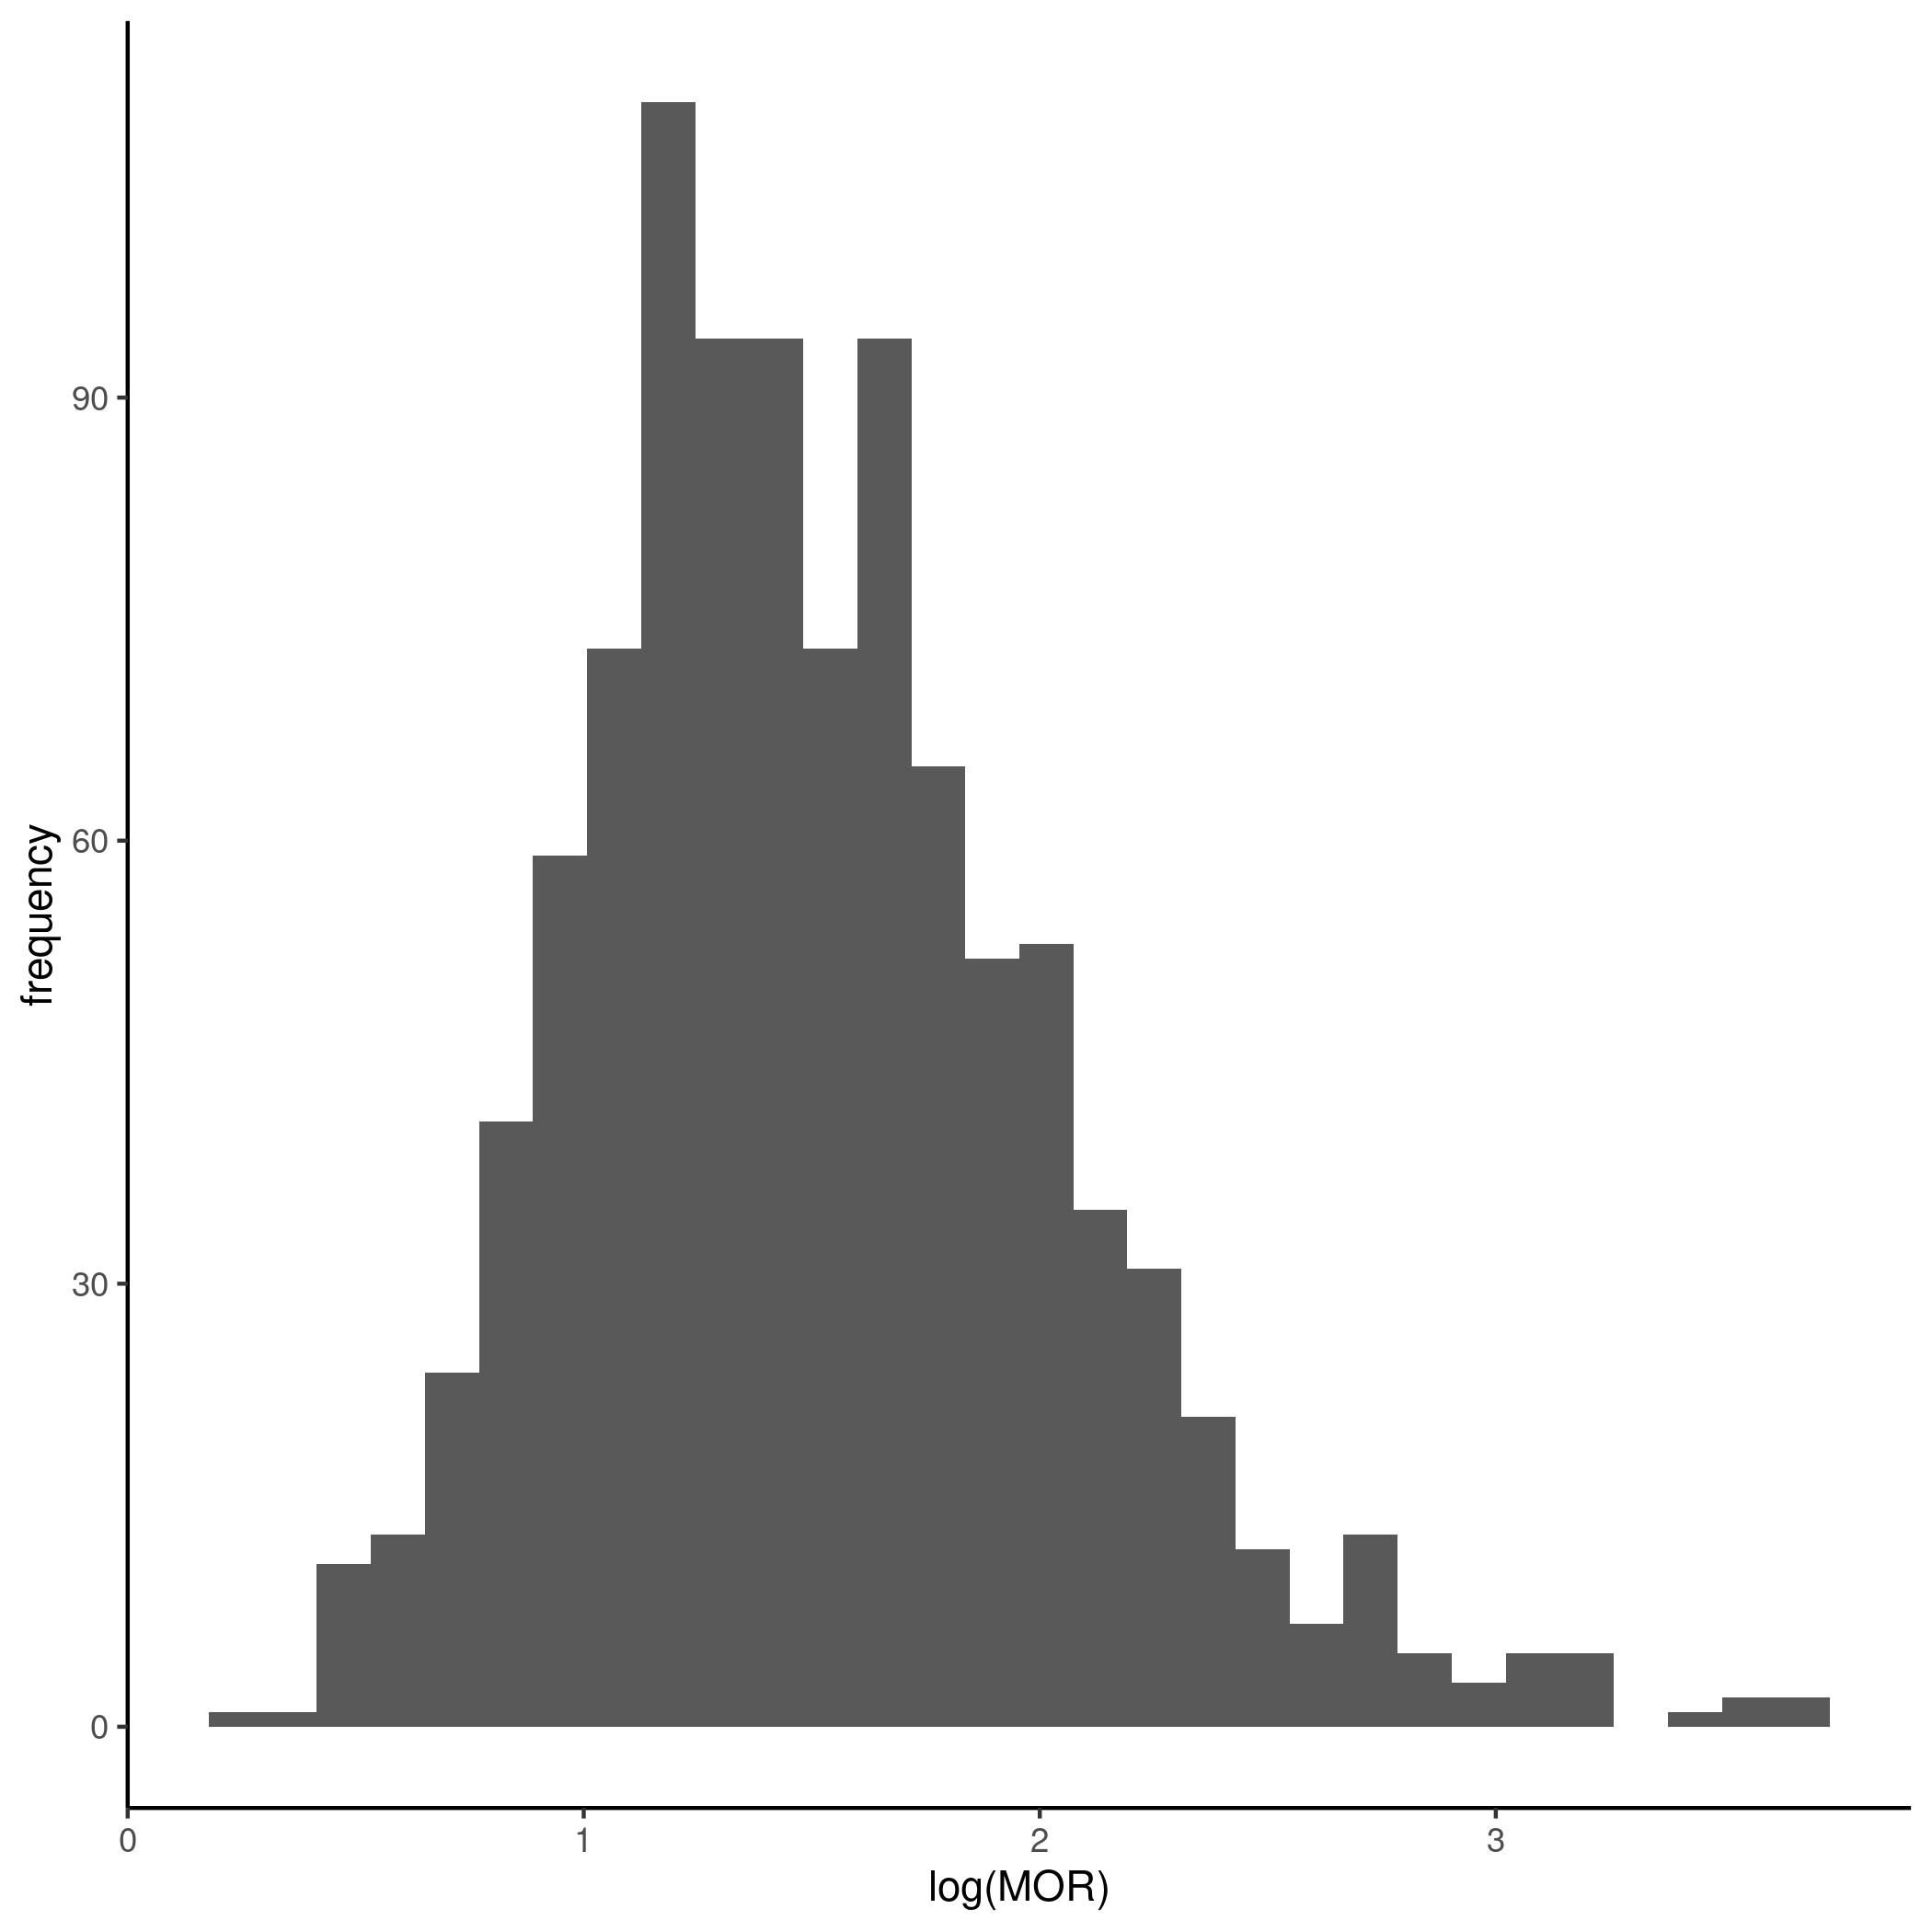
\includegraphics{../../plots/two-lvl-ran-int/high-prev/hist_30_5_two_lvl_high_prev.png}

}

\caption{Cluster size 5}

}

\end{minipage}%
%
\begin{minipage}[t]{0.24\linewidth}

{\centering 

\raisebox{-\height}{

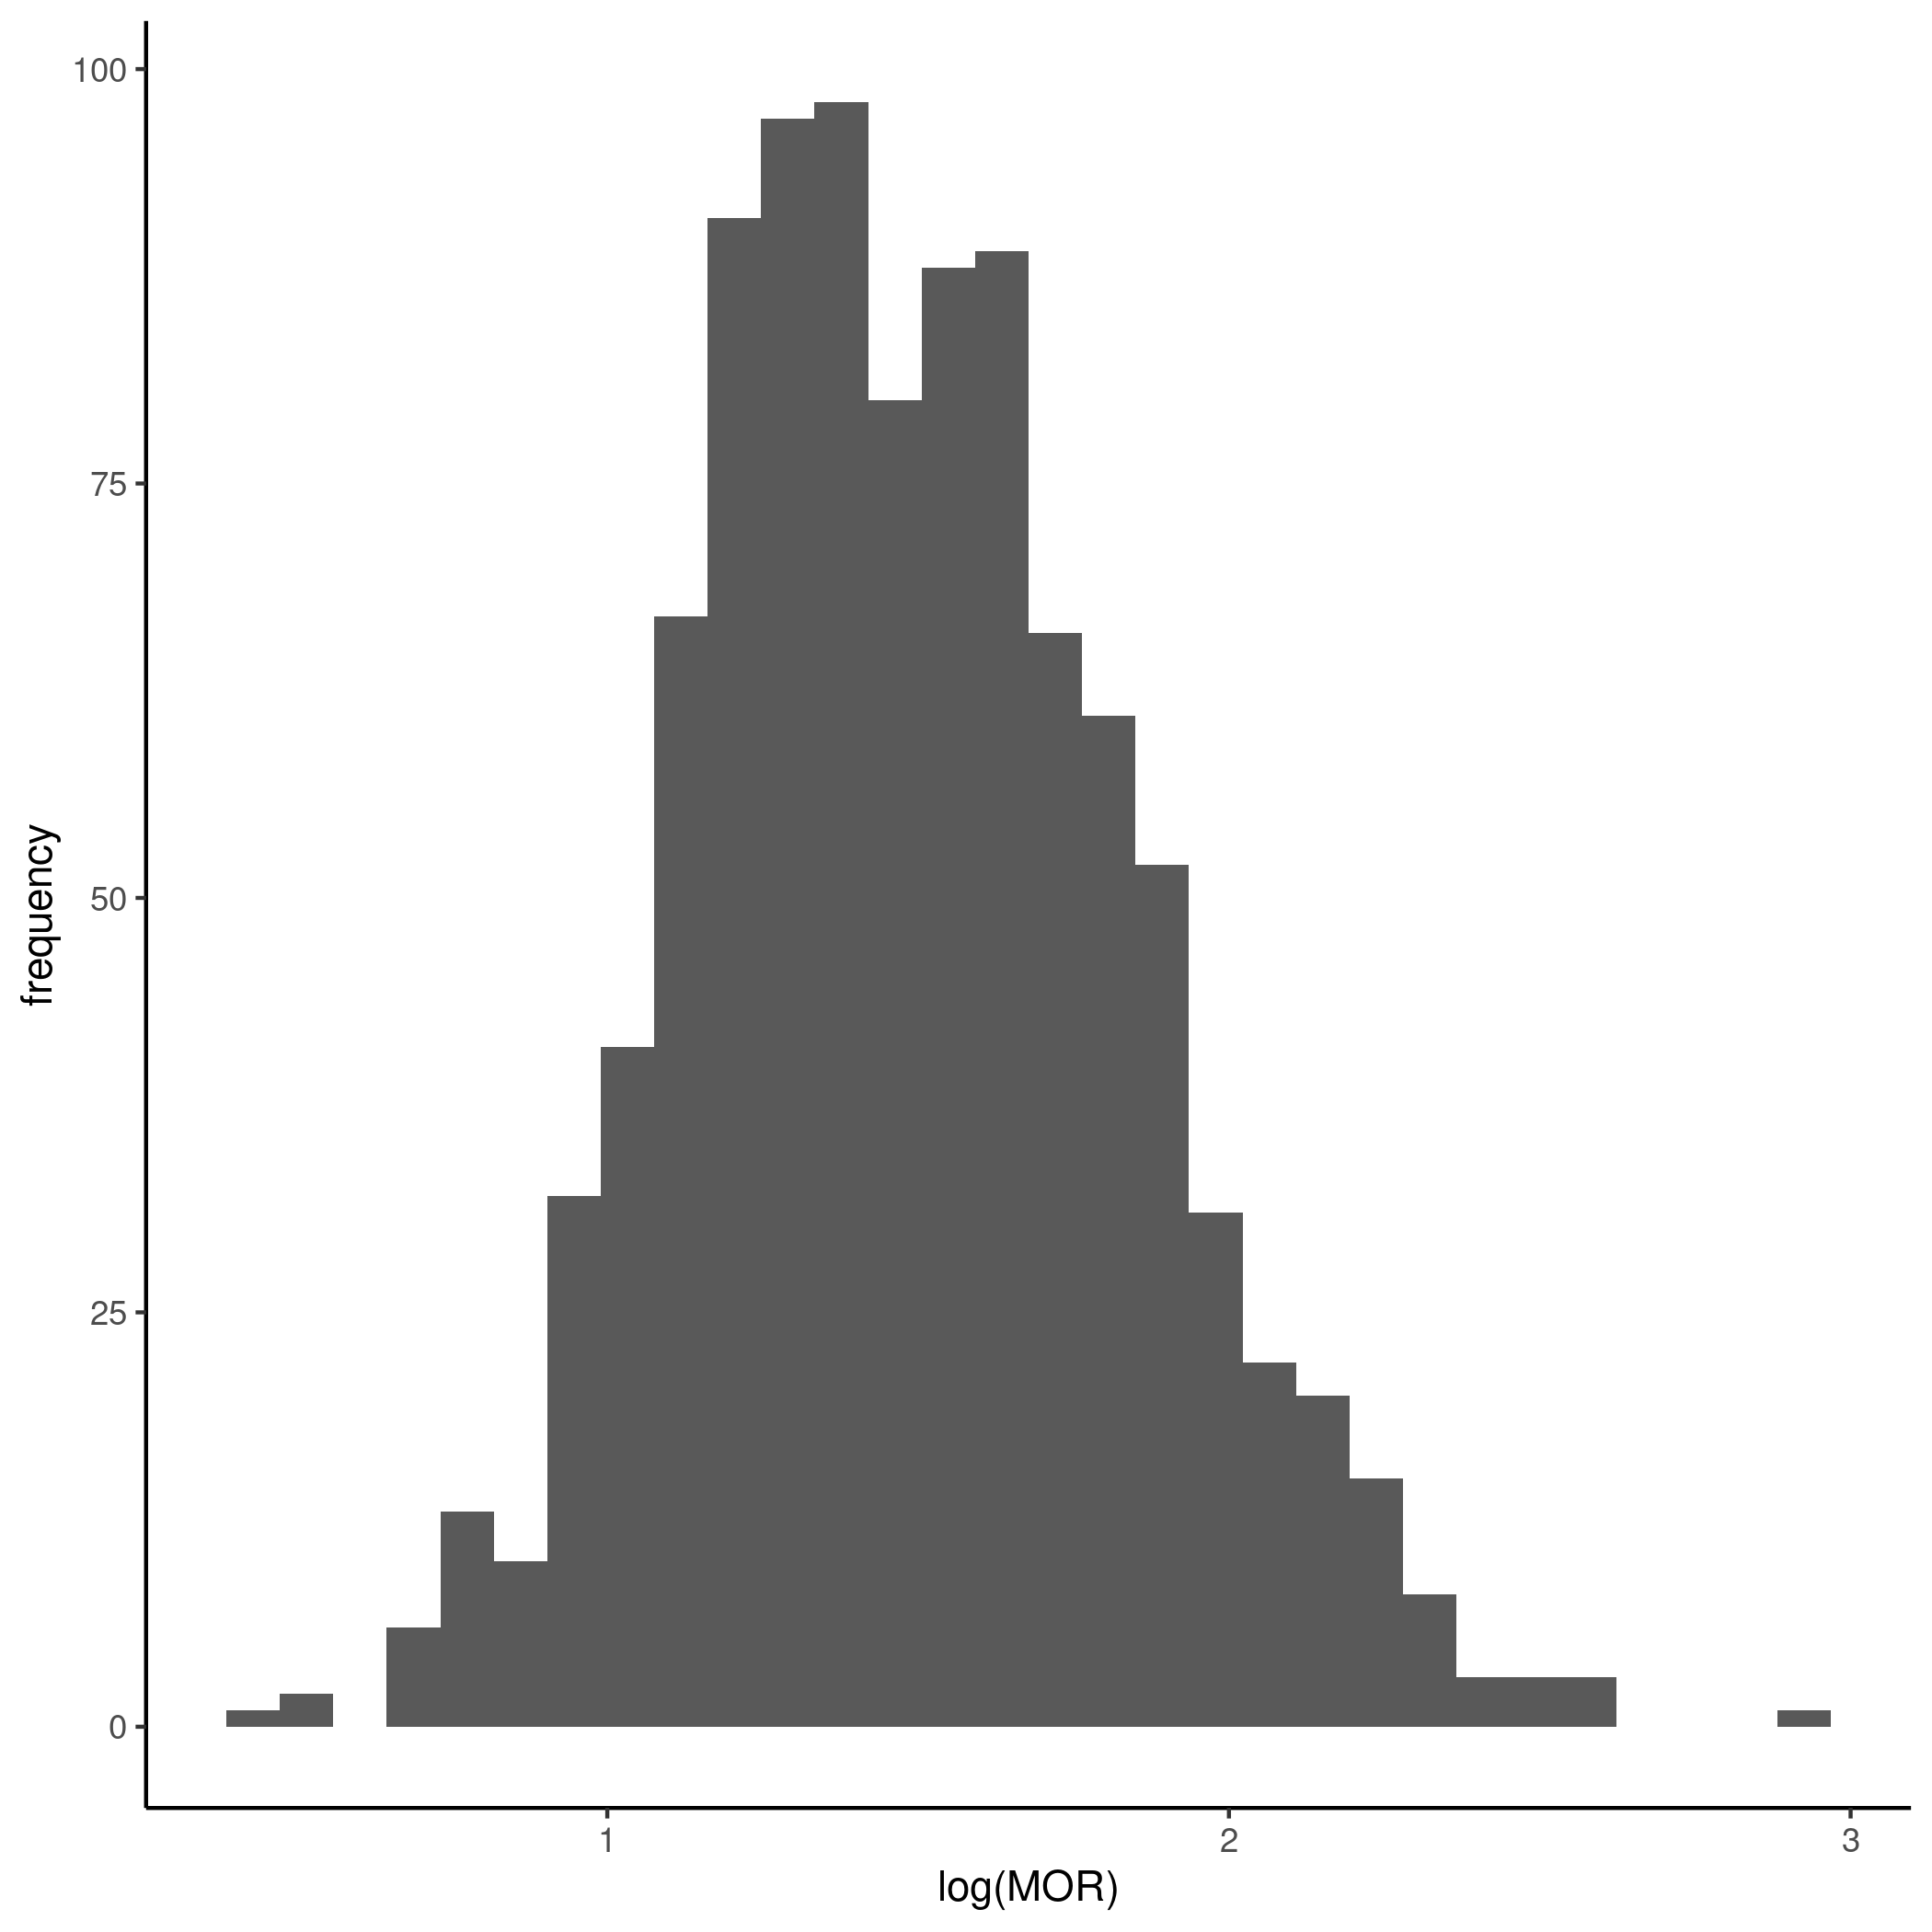
\includegraphics{../../plots/two-lvl-ran-int/high-prev/hist_30_10_two_lvl_high_prev.png}

}

\caption{Cluster size 10}

}

\end{minipage}%
%
\begin{minipage}[t]{0.24\linewidth}

{\centering 

\raisebox{-\height}{

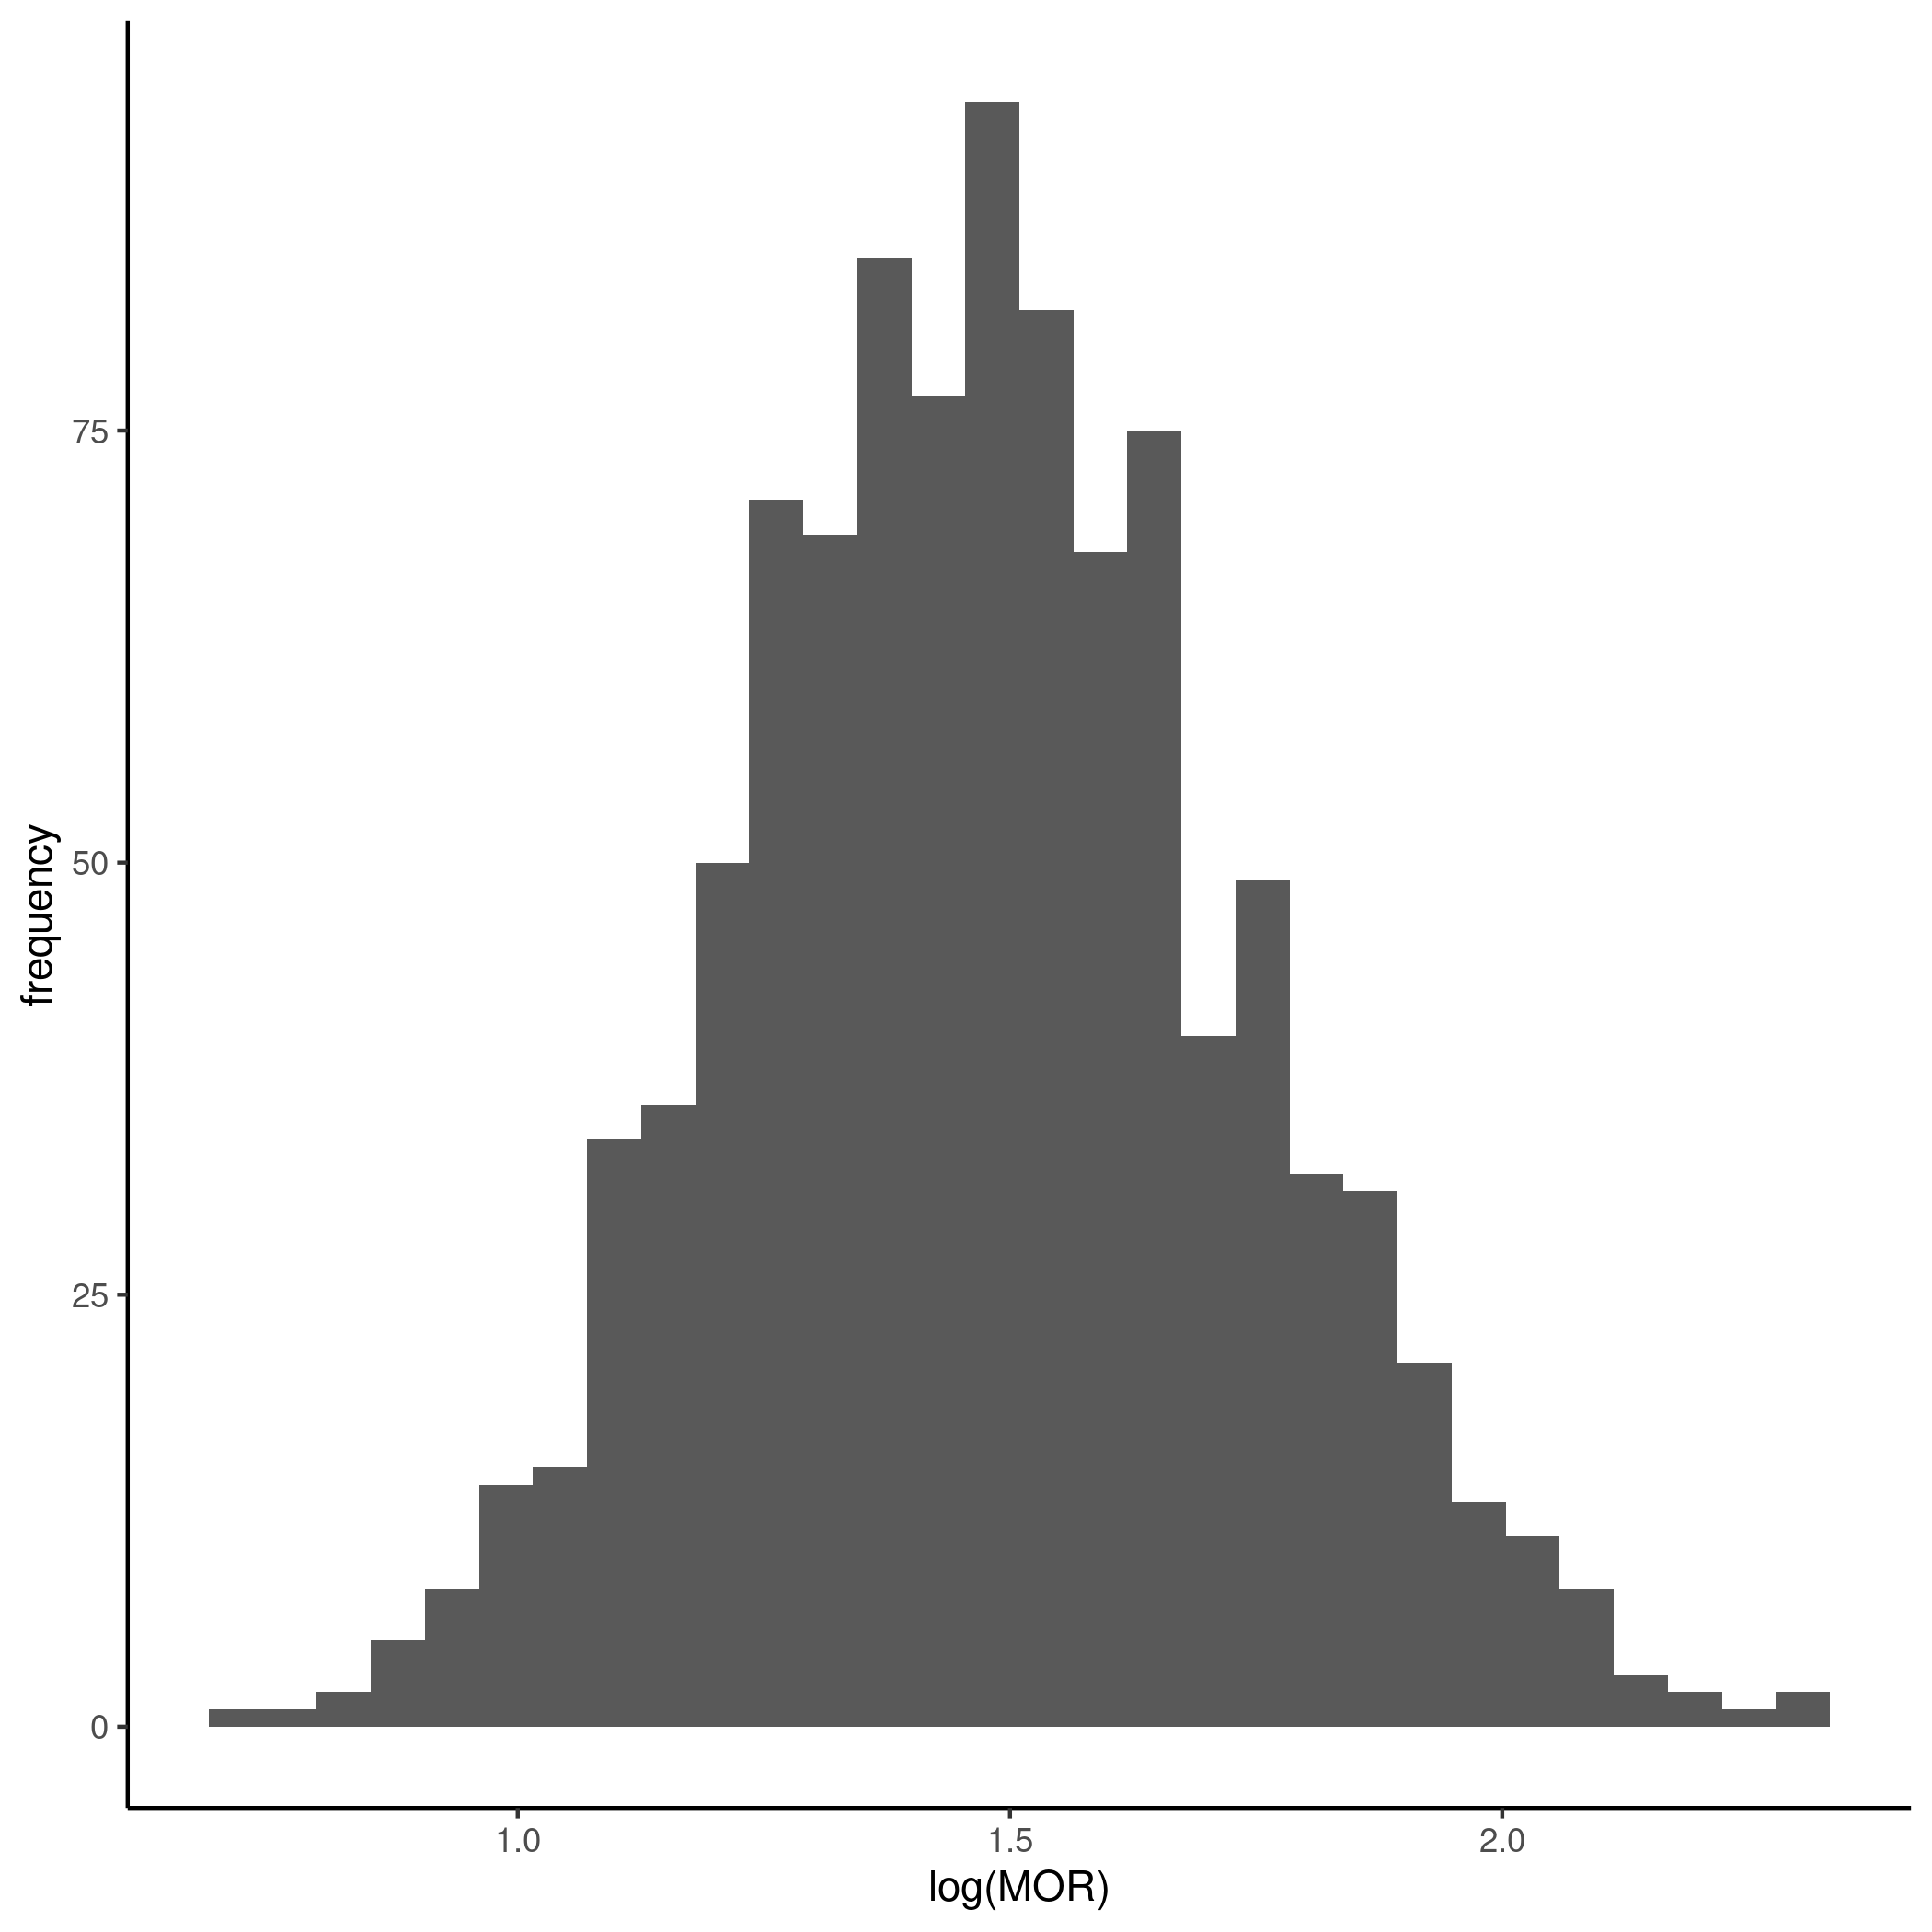
\includegraphics{../../plots/two-lvl-ran-int/high-prev/hist_30_30_two_lvl_high_prev.png}

}

\caption{Cluster size 30}

}

\end{minipage}%
%
\begin{minipage}[t]{0.24\linewidth}

{\centering 

\raisebox{-\height}{

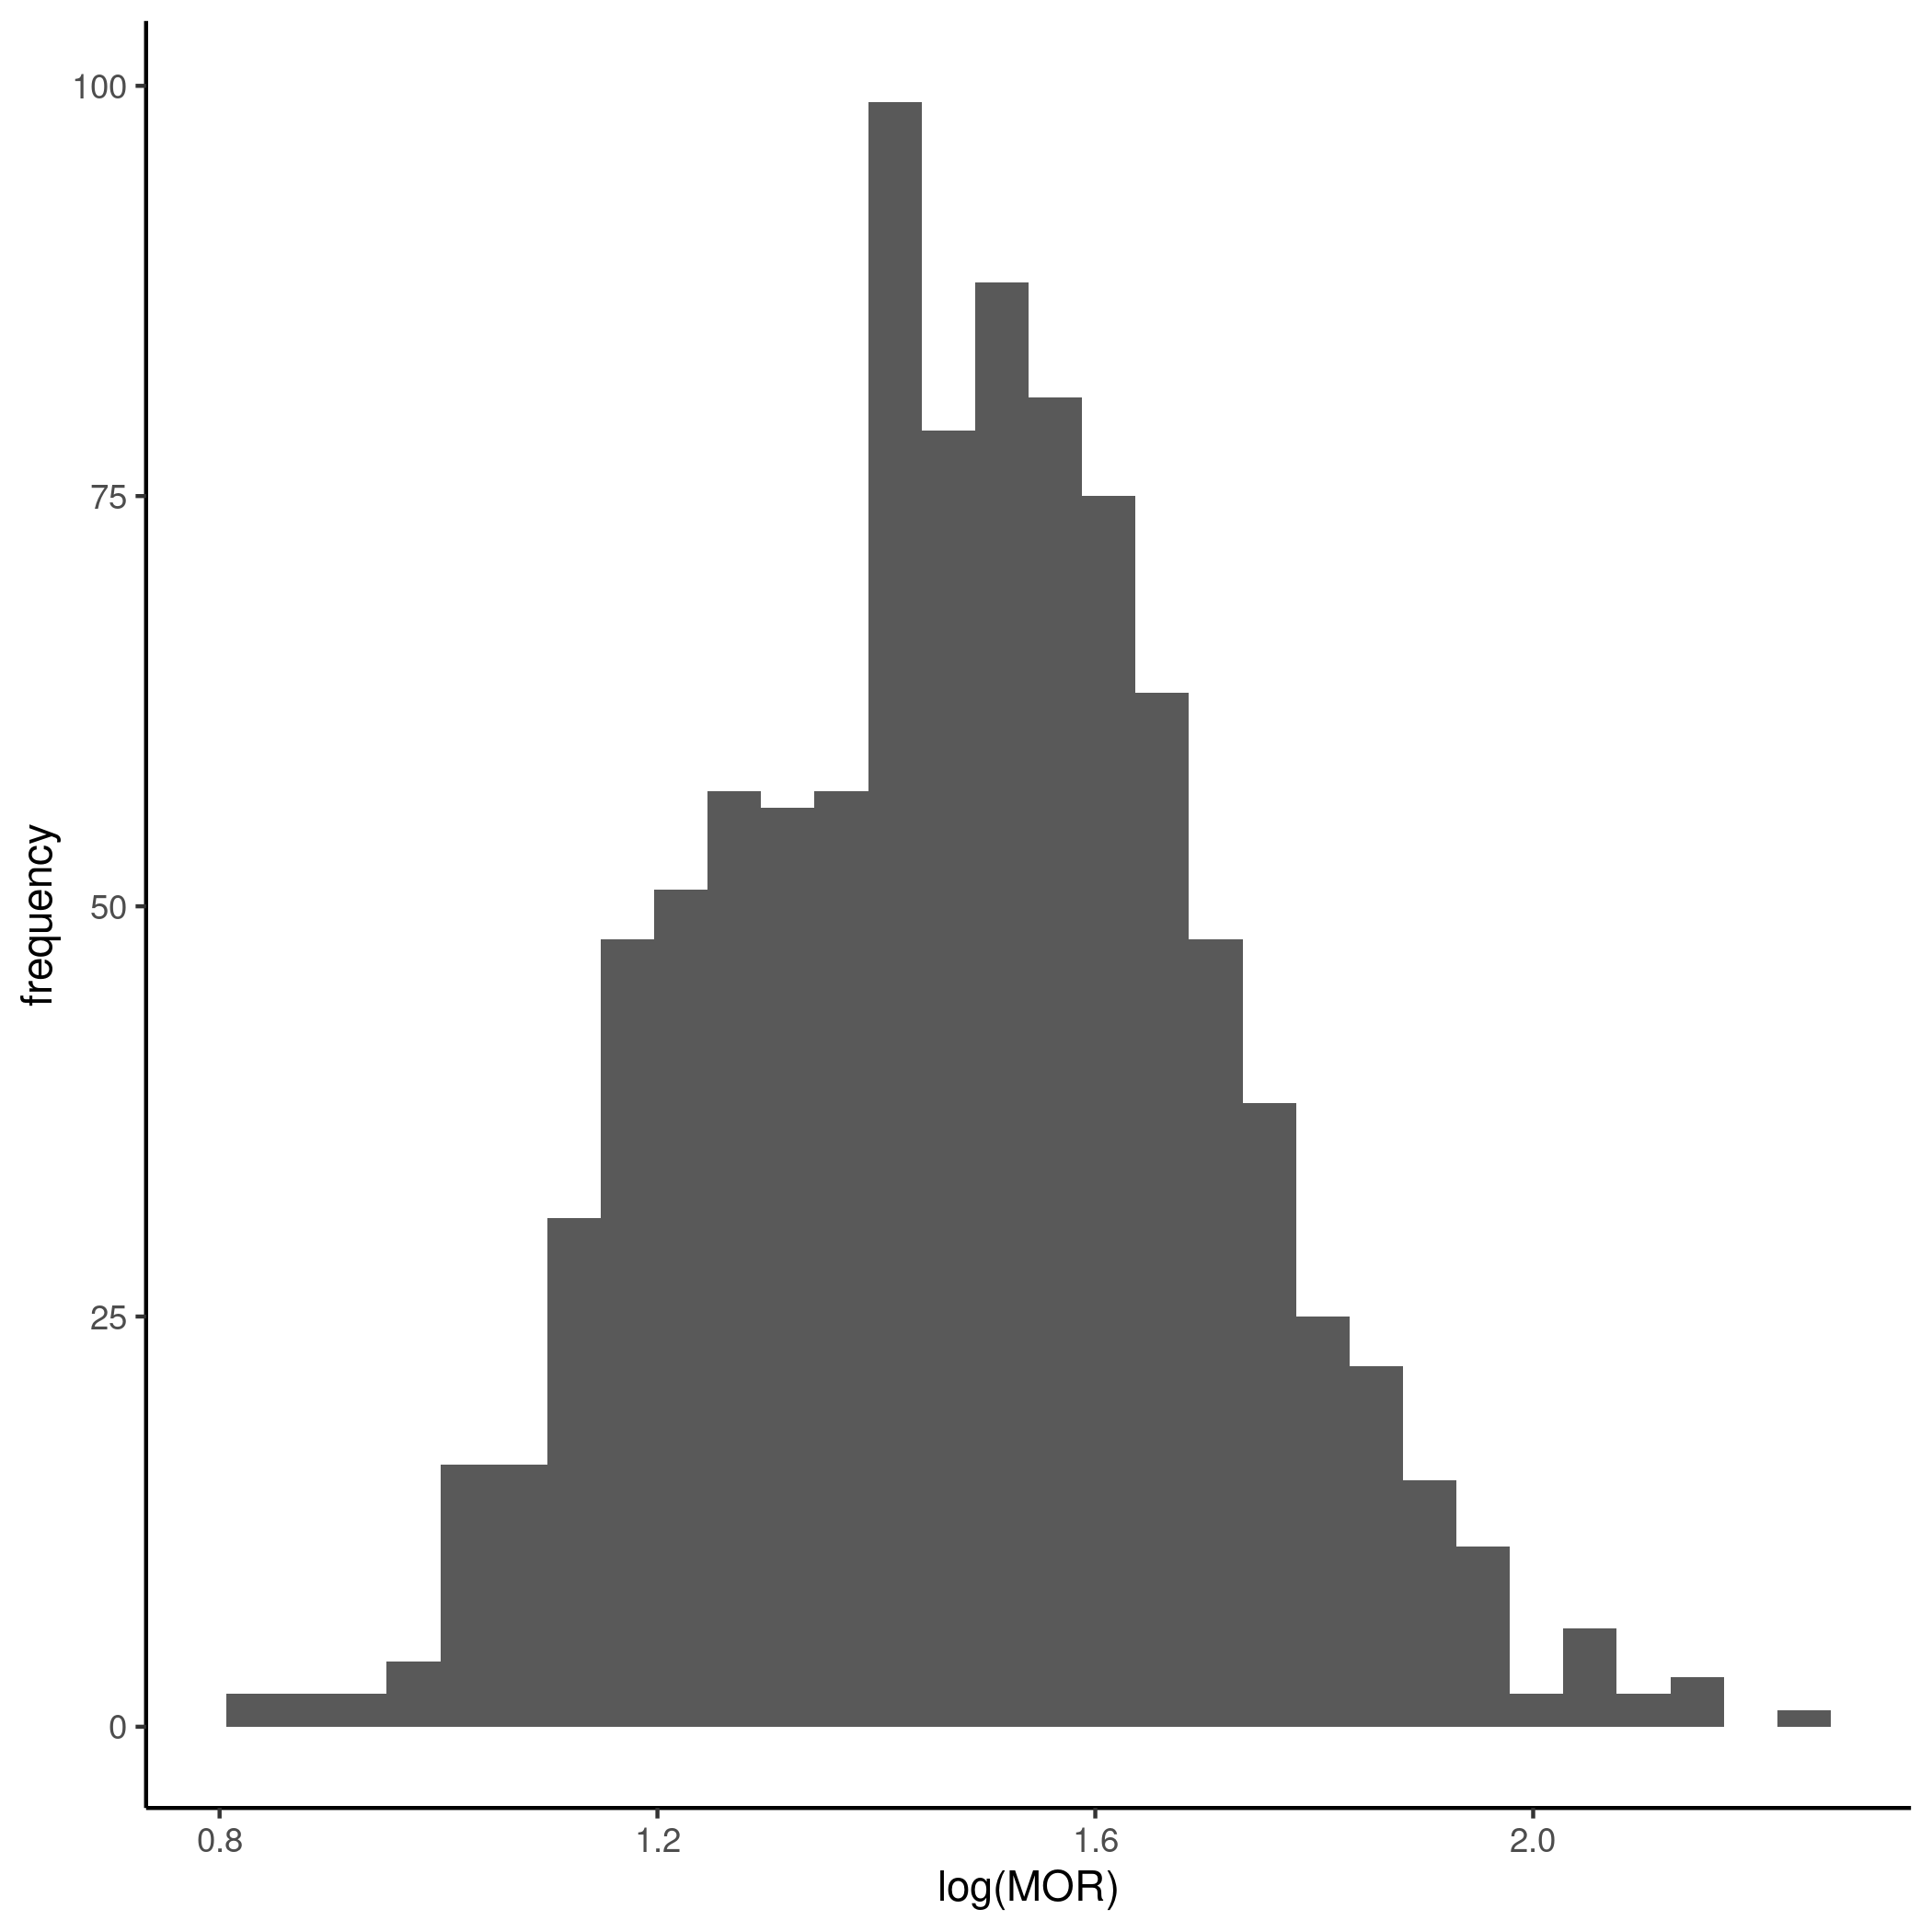
\includegraphics{../../plots/two-lvl-ran-int/high-prev/hist_30_50_two_lvl_high_prev.png}

}

\caption{Cluster size 50}

}

\end{minipage}%
\newline
\begin{minipage}[t]{\linewidth}

{\centering 

~

}

\end{minipage}%
\newline
\begin{minipage}[t]{0.05\linewidth}

{\centering 

\rotatebox[origin=br]{90}{\tiny Cluster Number 50}

}

\end{minipage}%
%
\begin{minipage}[t]{0.24\linewidth}

{\centering 

\raisebox{-\height}{

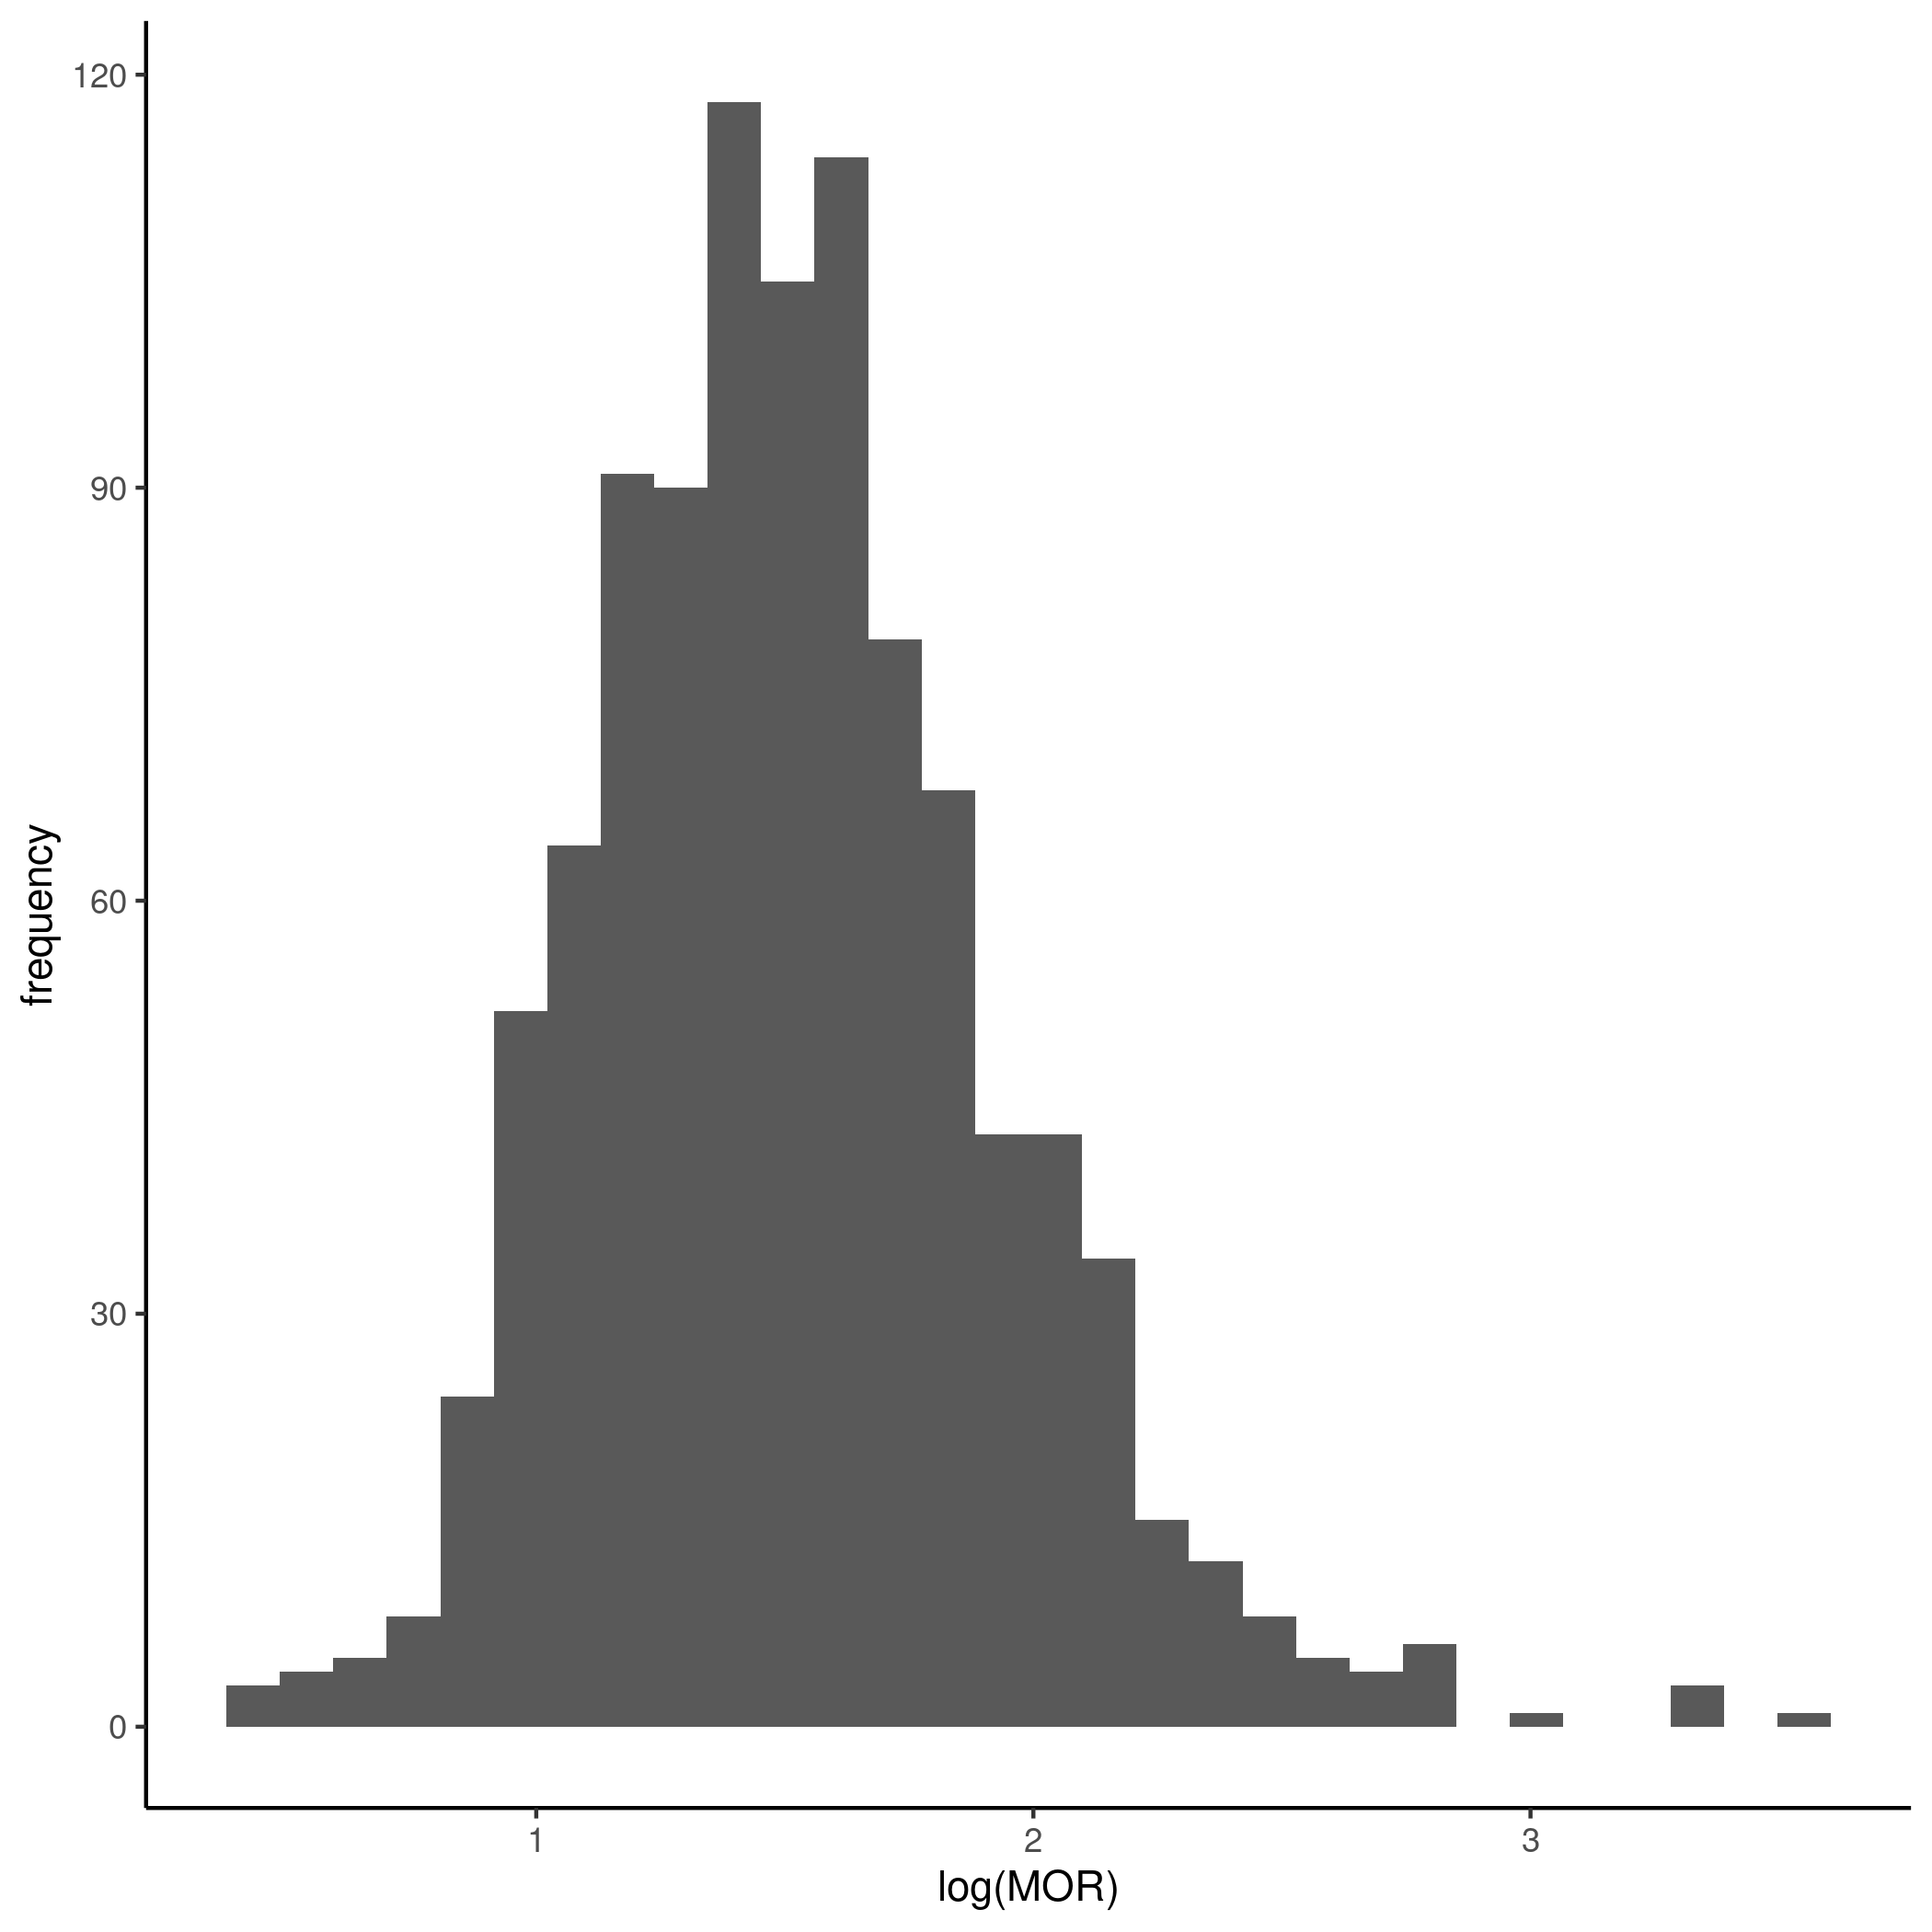
\includegraphics{../../plots/two-lvl-ran-int/high-prev/hist_50_5_two_lvl_high_prev.png}

}

\caption{Cluster size 5}

}

\end{minipage}%
%
\begin{minipage}[t]{0.24\linewidth}

{\centering 

\raisebox{-\height}{

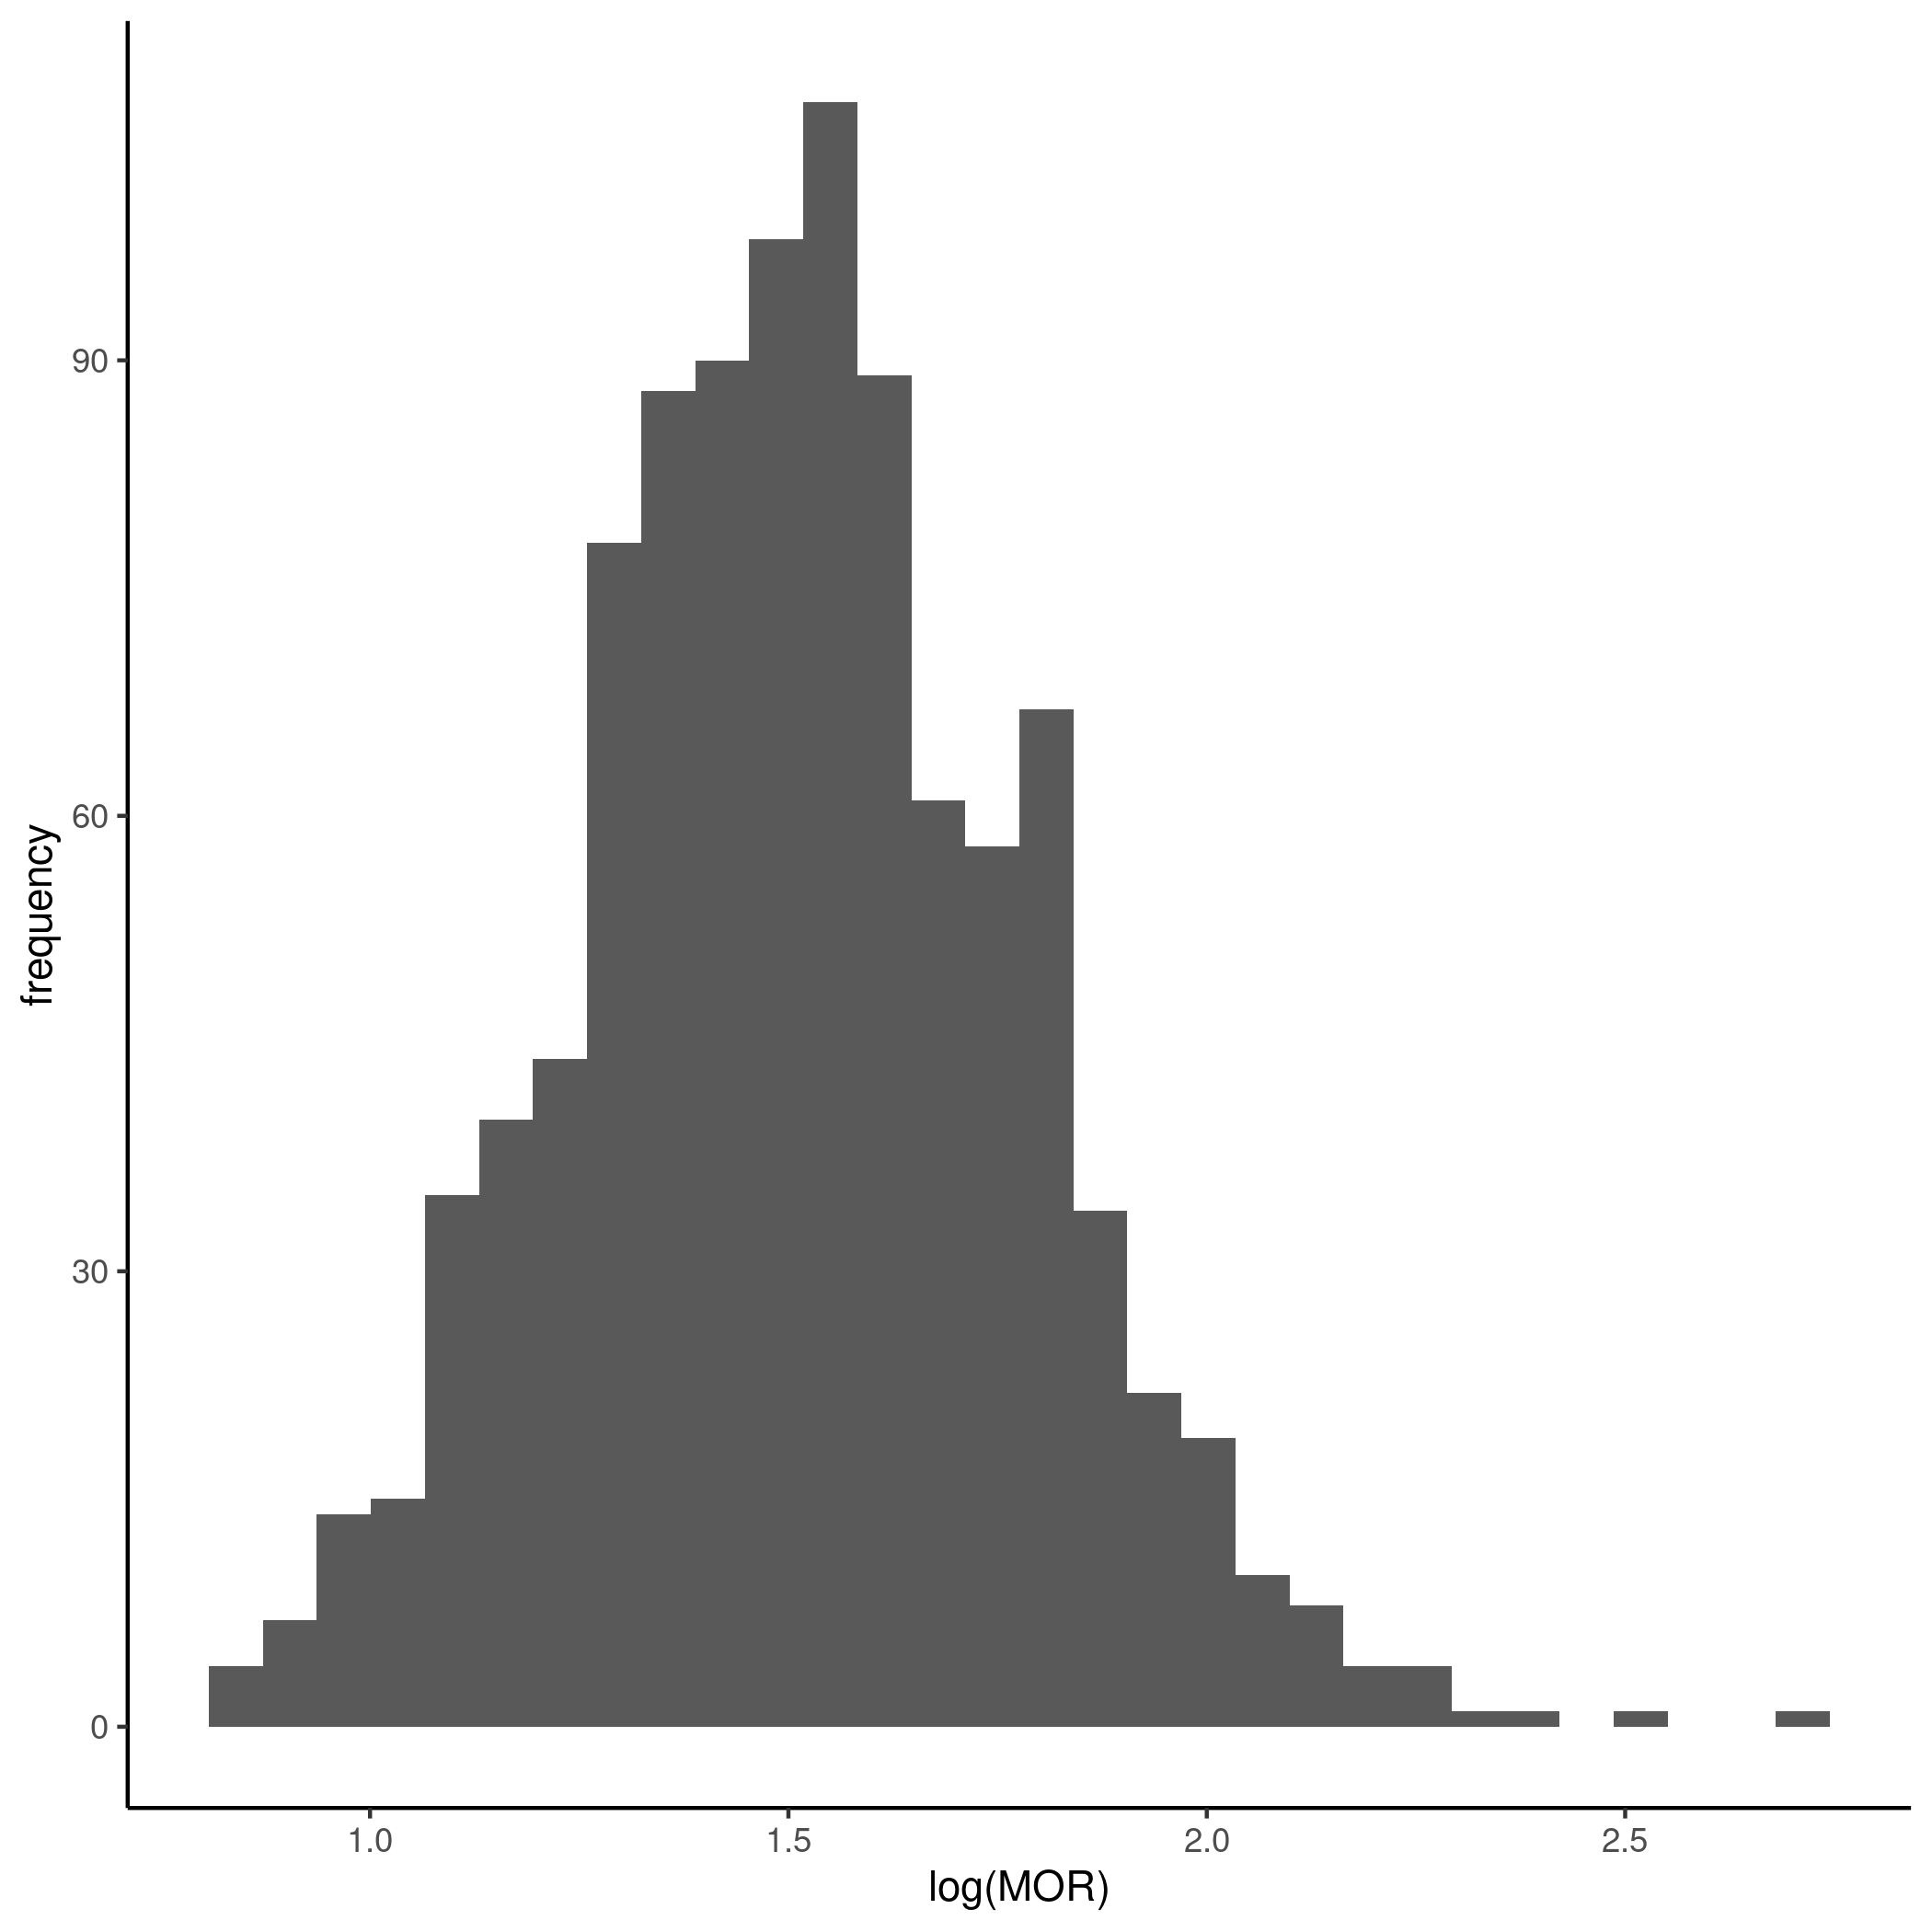
\includegraphics{../../plots/two-lvl-ran-int/high-prev/hist_50_10_two_lvl_high_prev.png}

}

\caption{Cluster size 10}

}

\end{minipage}%
%
\begin{minipage}[t]{0.24\linewidth}

{\centering 

\raisebox{-\height}{

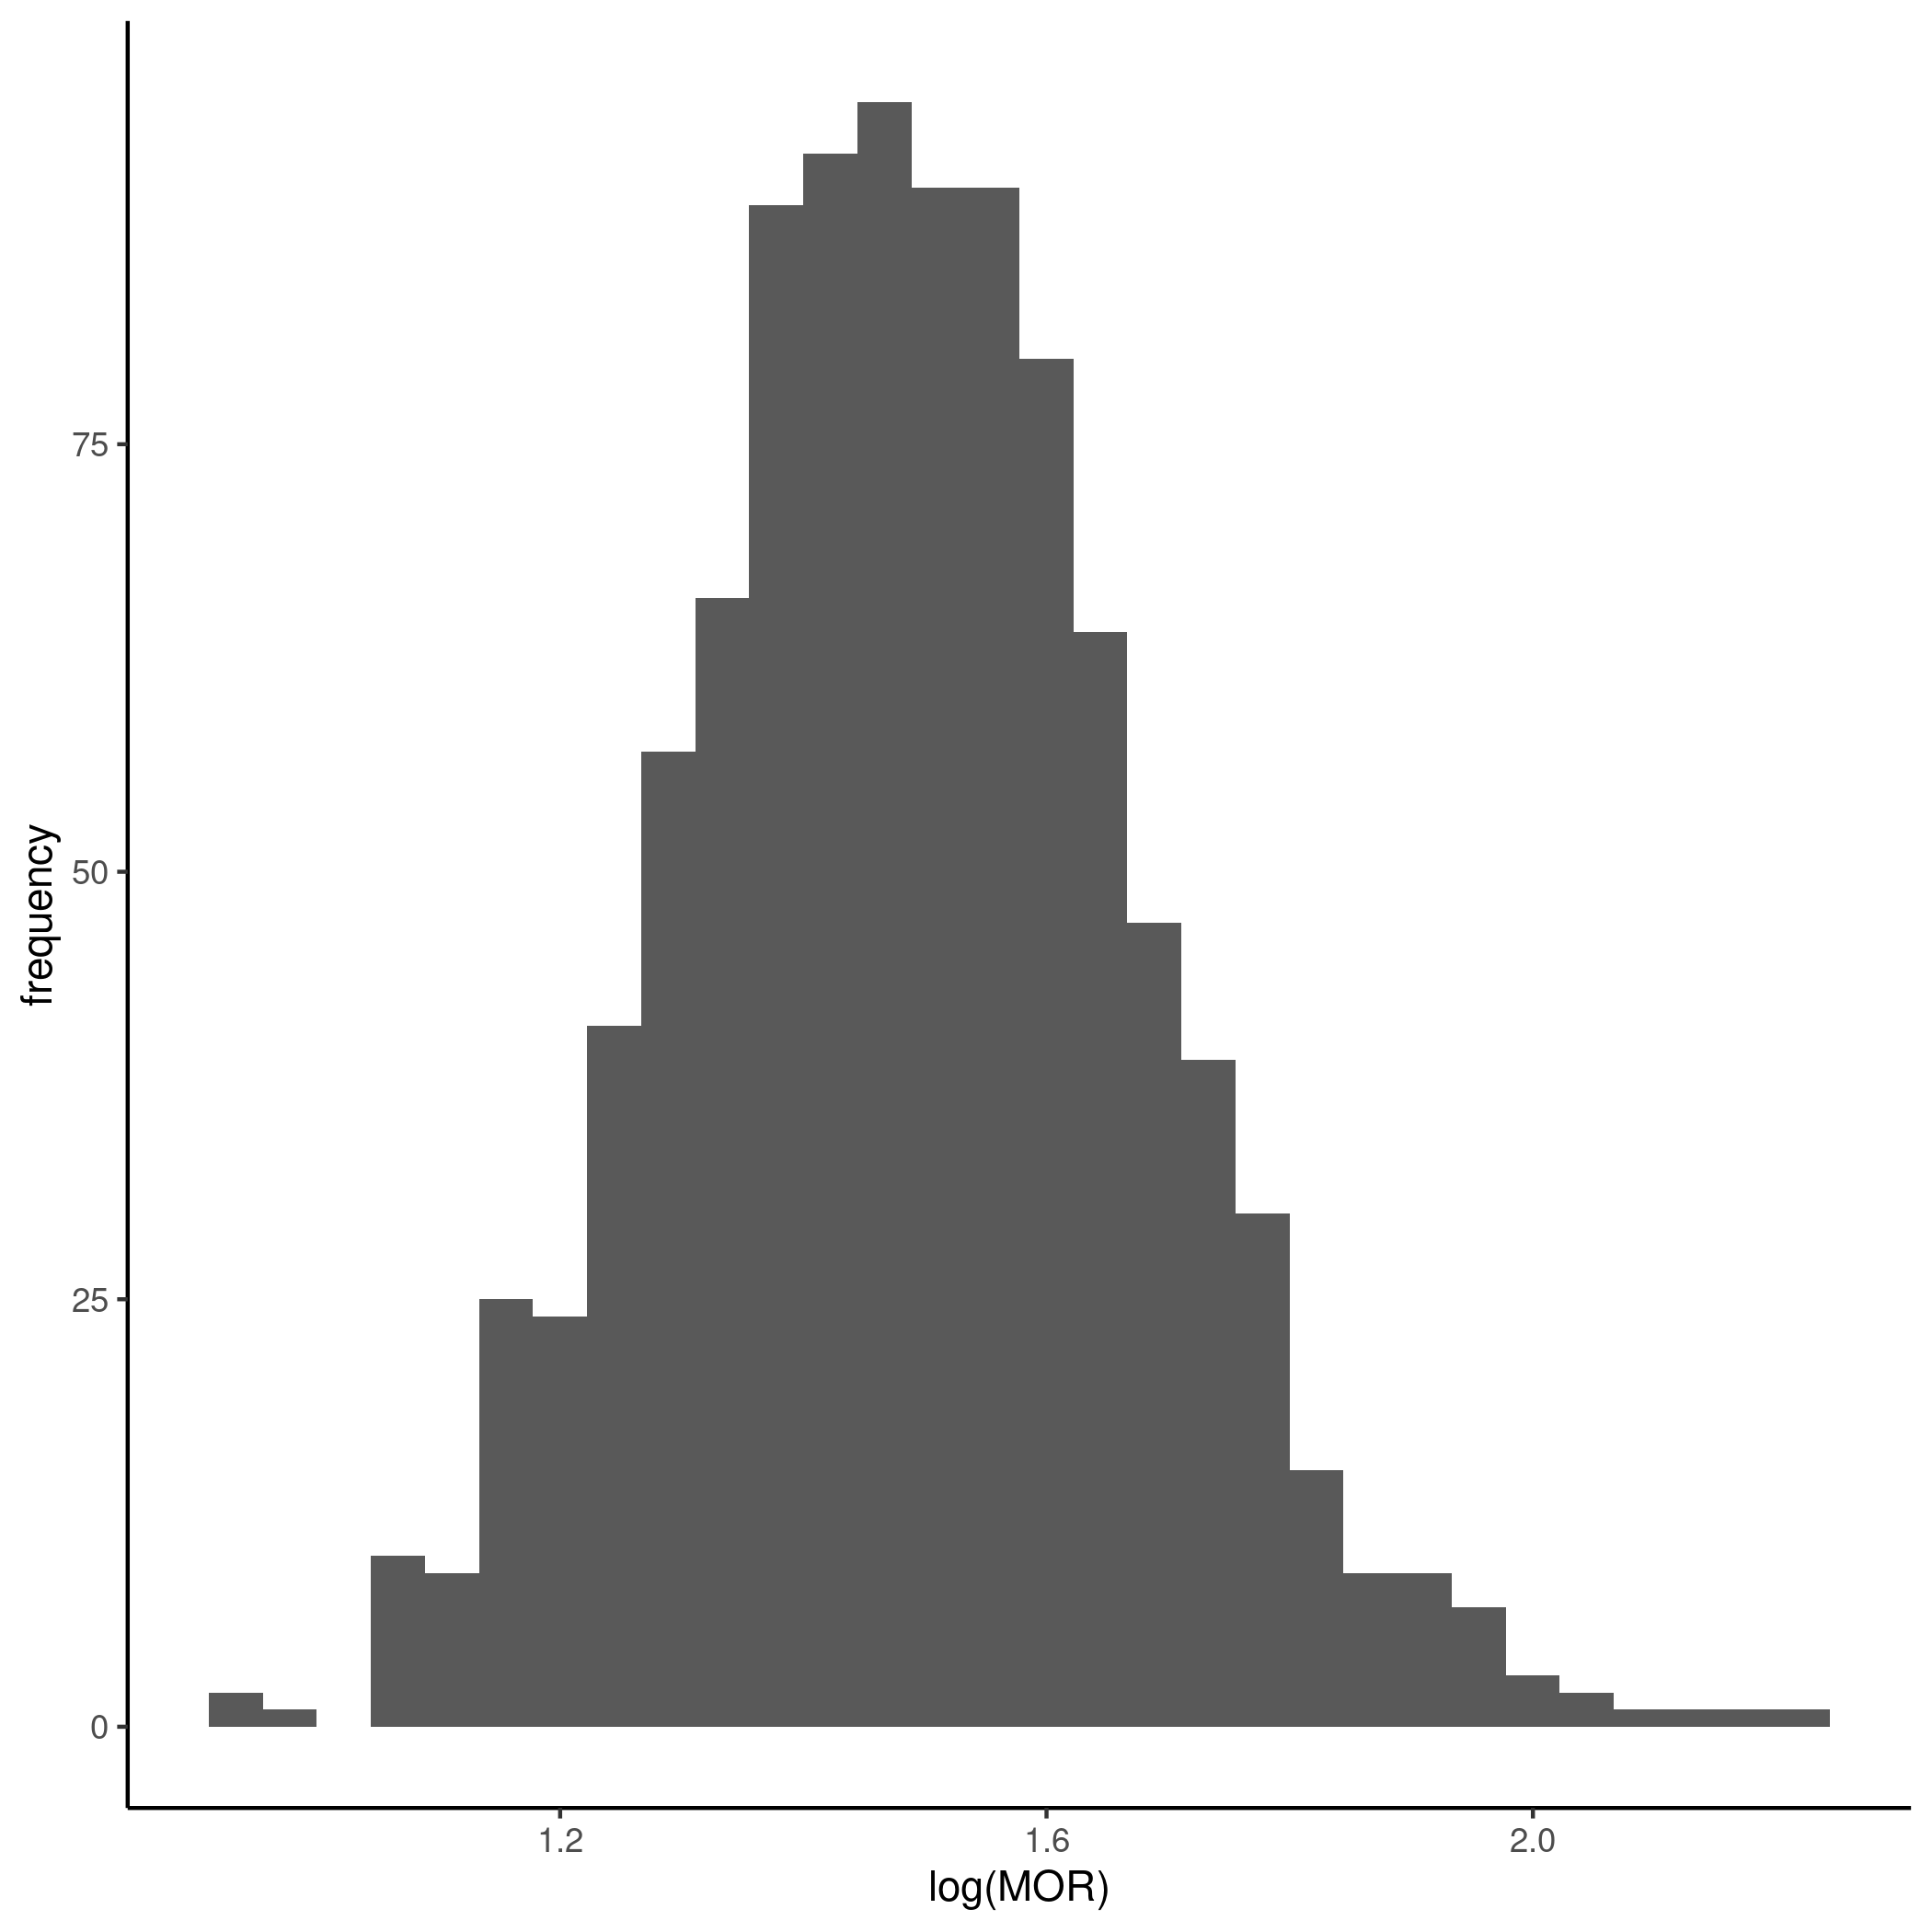
\includegraphics{../../plots/two-lvl-ran-int/high-prev/hist_50_30_two_lvl_high_prev.png}

}

\caption{Cluster size 30}

}

\end{minipage}%
%
\begin{minipage}[t]{0.24\linewidth}

{\centering 

\raisebox{-\height}{

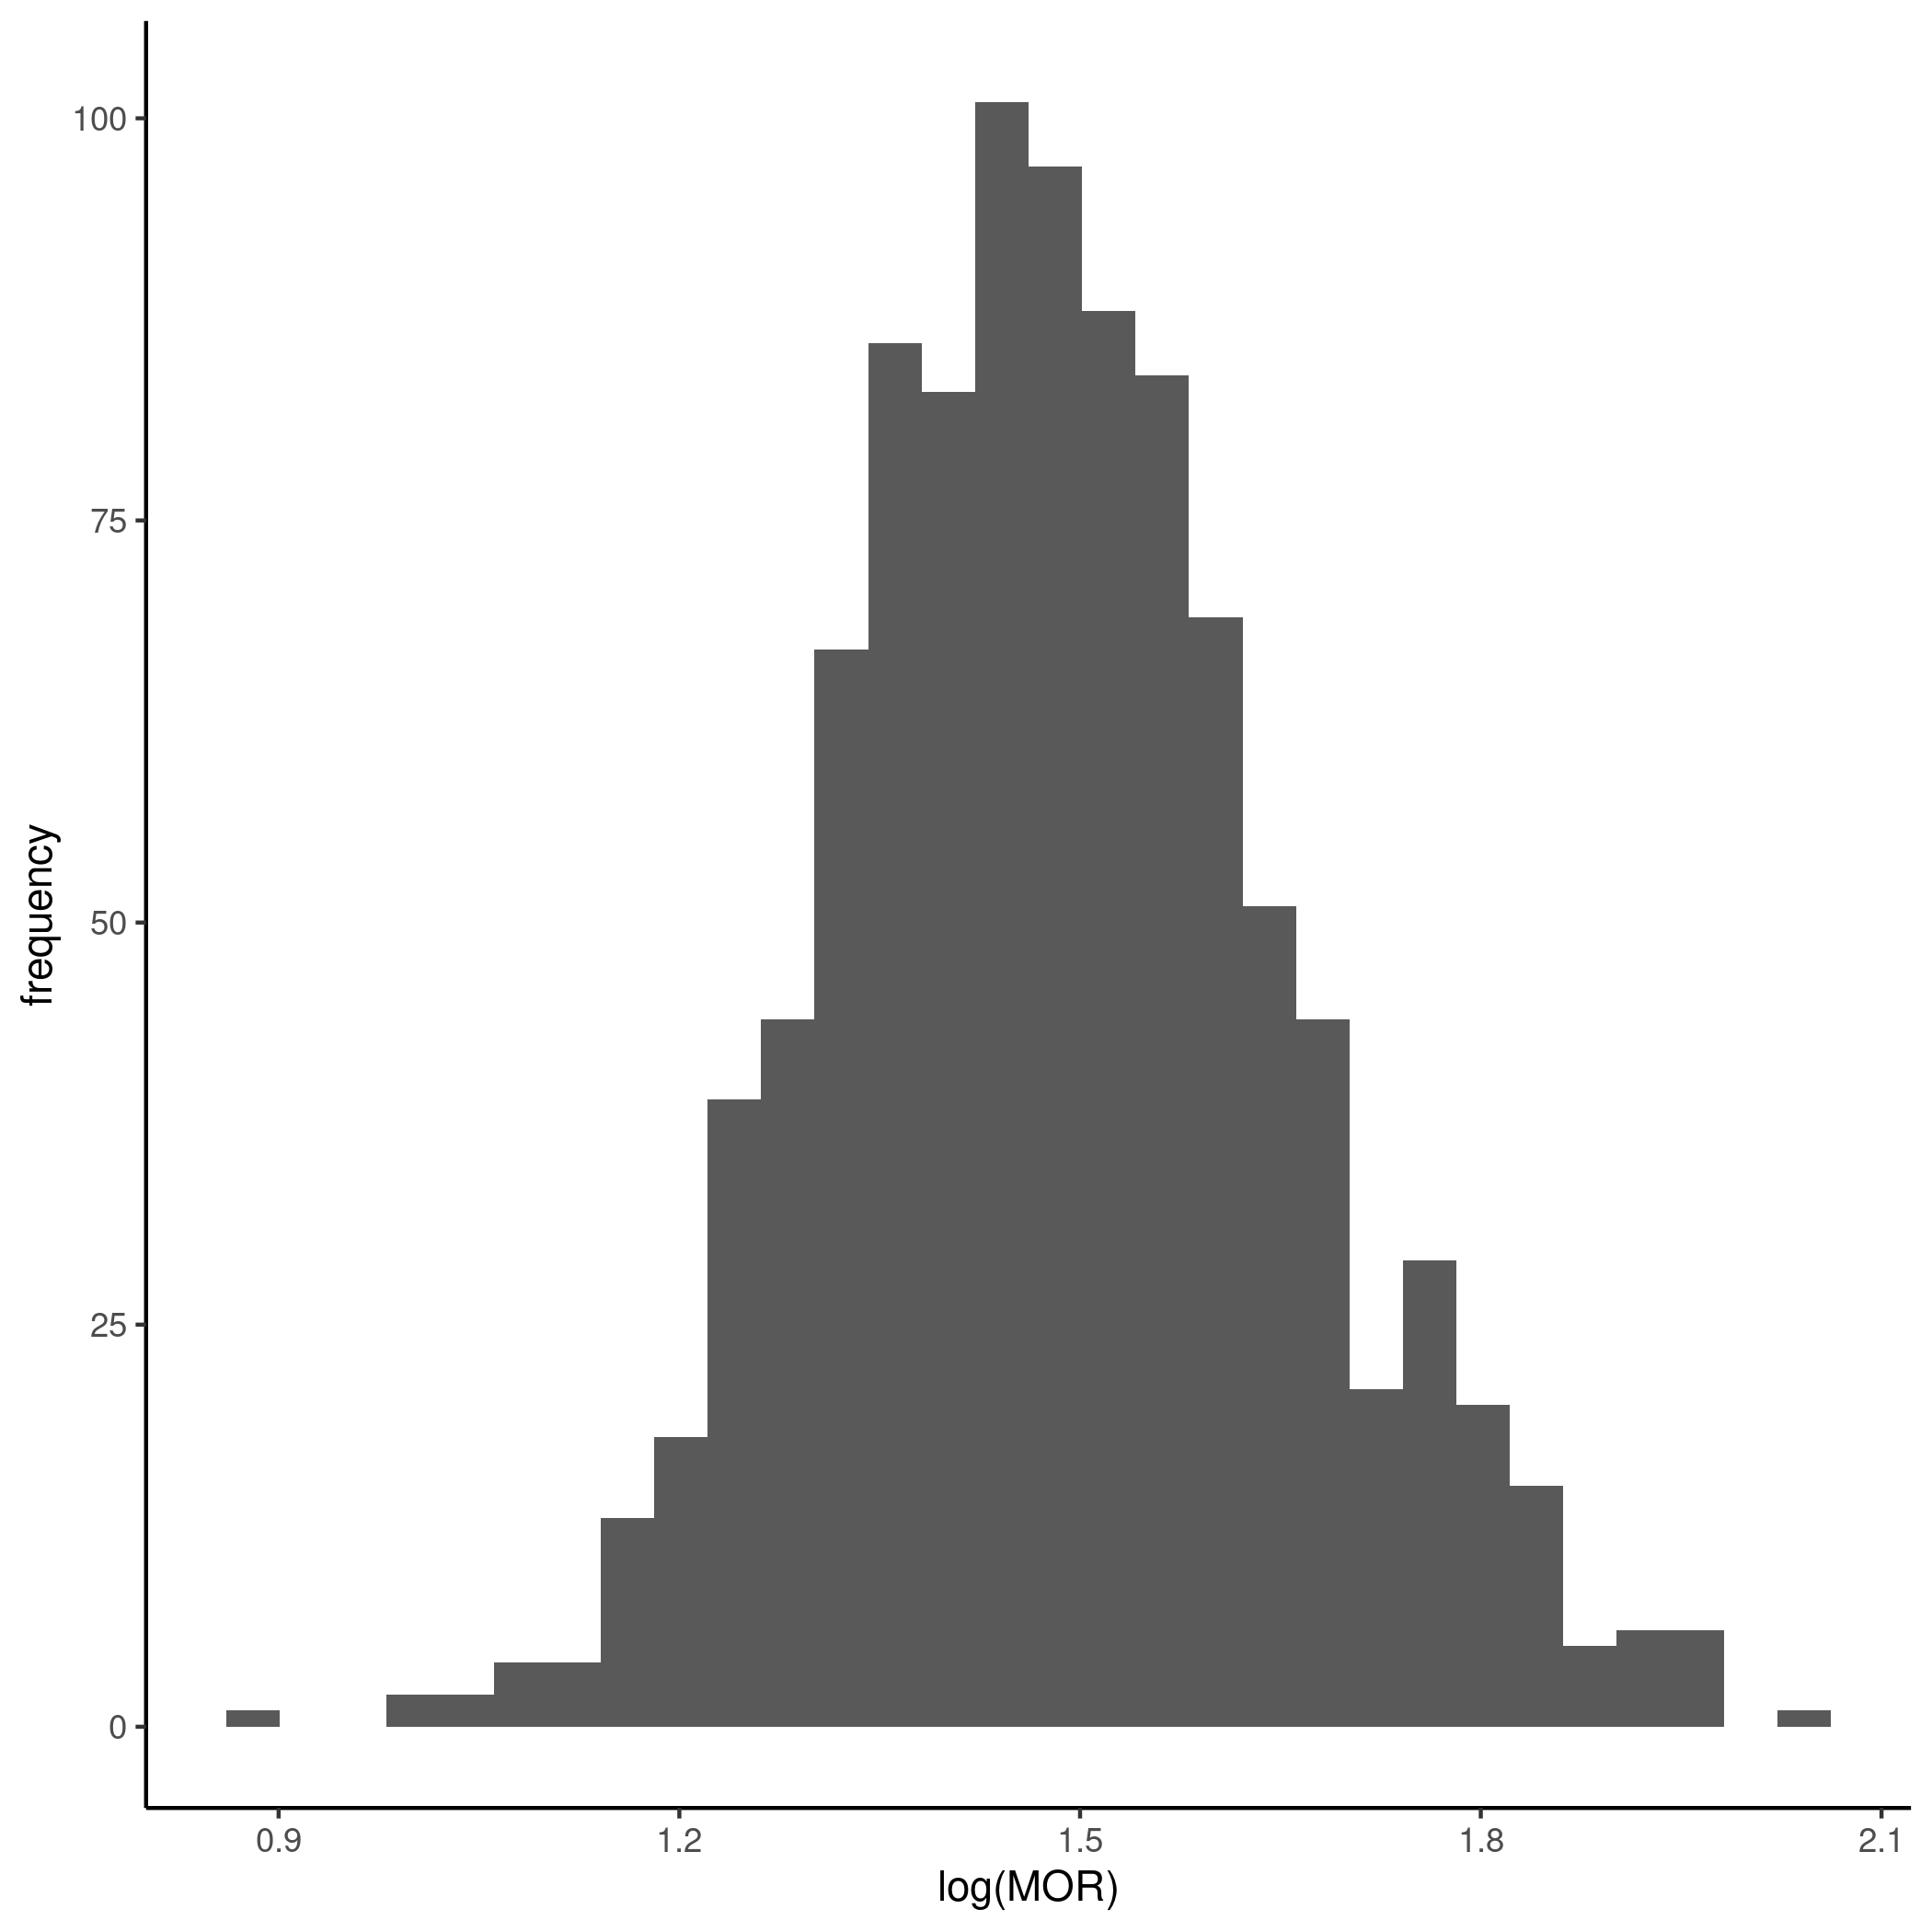
\includegraphics{../../plots/two-lvl-ran-int/high-prev/hist_50_50_two_lvl_high_prev.png}

}

\caption{Cluster size 50}

}

\end{minipage}%
\newline
\begin{minipage}[t]{\linewidth}

{\centering 

~

}

\end{minipage}%
\newline
\begin{minipage}[t]{0.05\linewidth}

{\centering 

\rotatebox[origin=br]{90}{\tiny Cluster Number 100}

}

\end{minipage}%
%
\begin{minipage}[t]{0.24\linewidth}

{\centering 

\raisebox{-\height}{

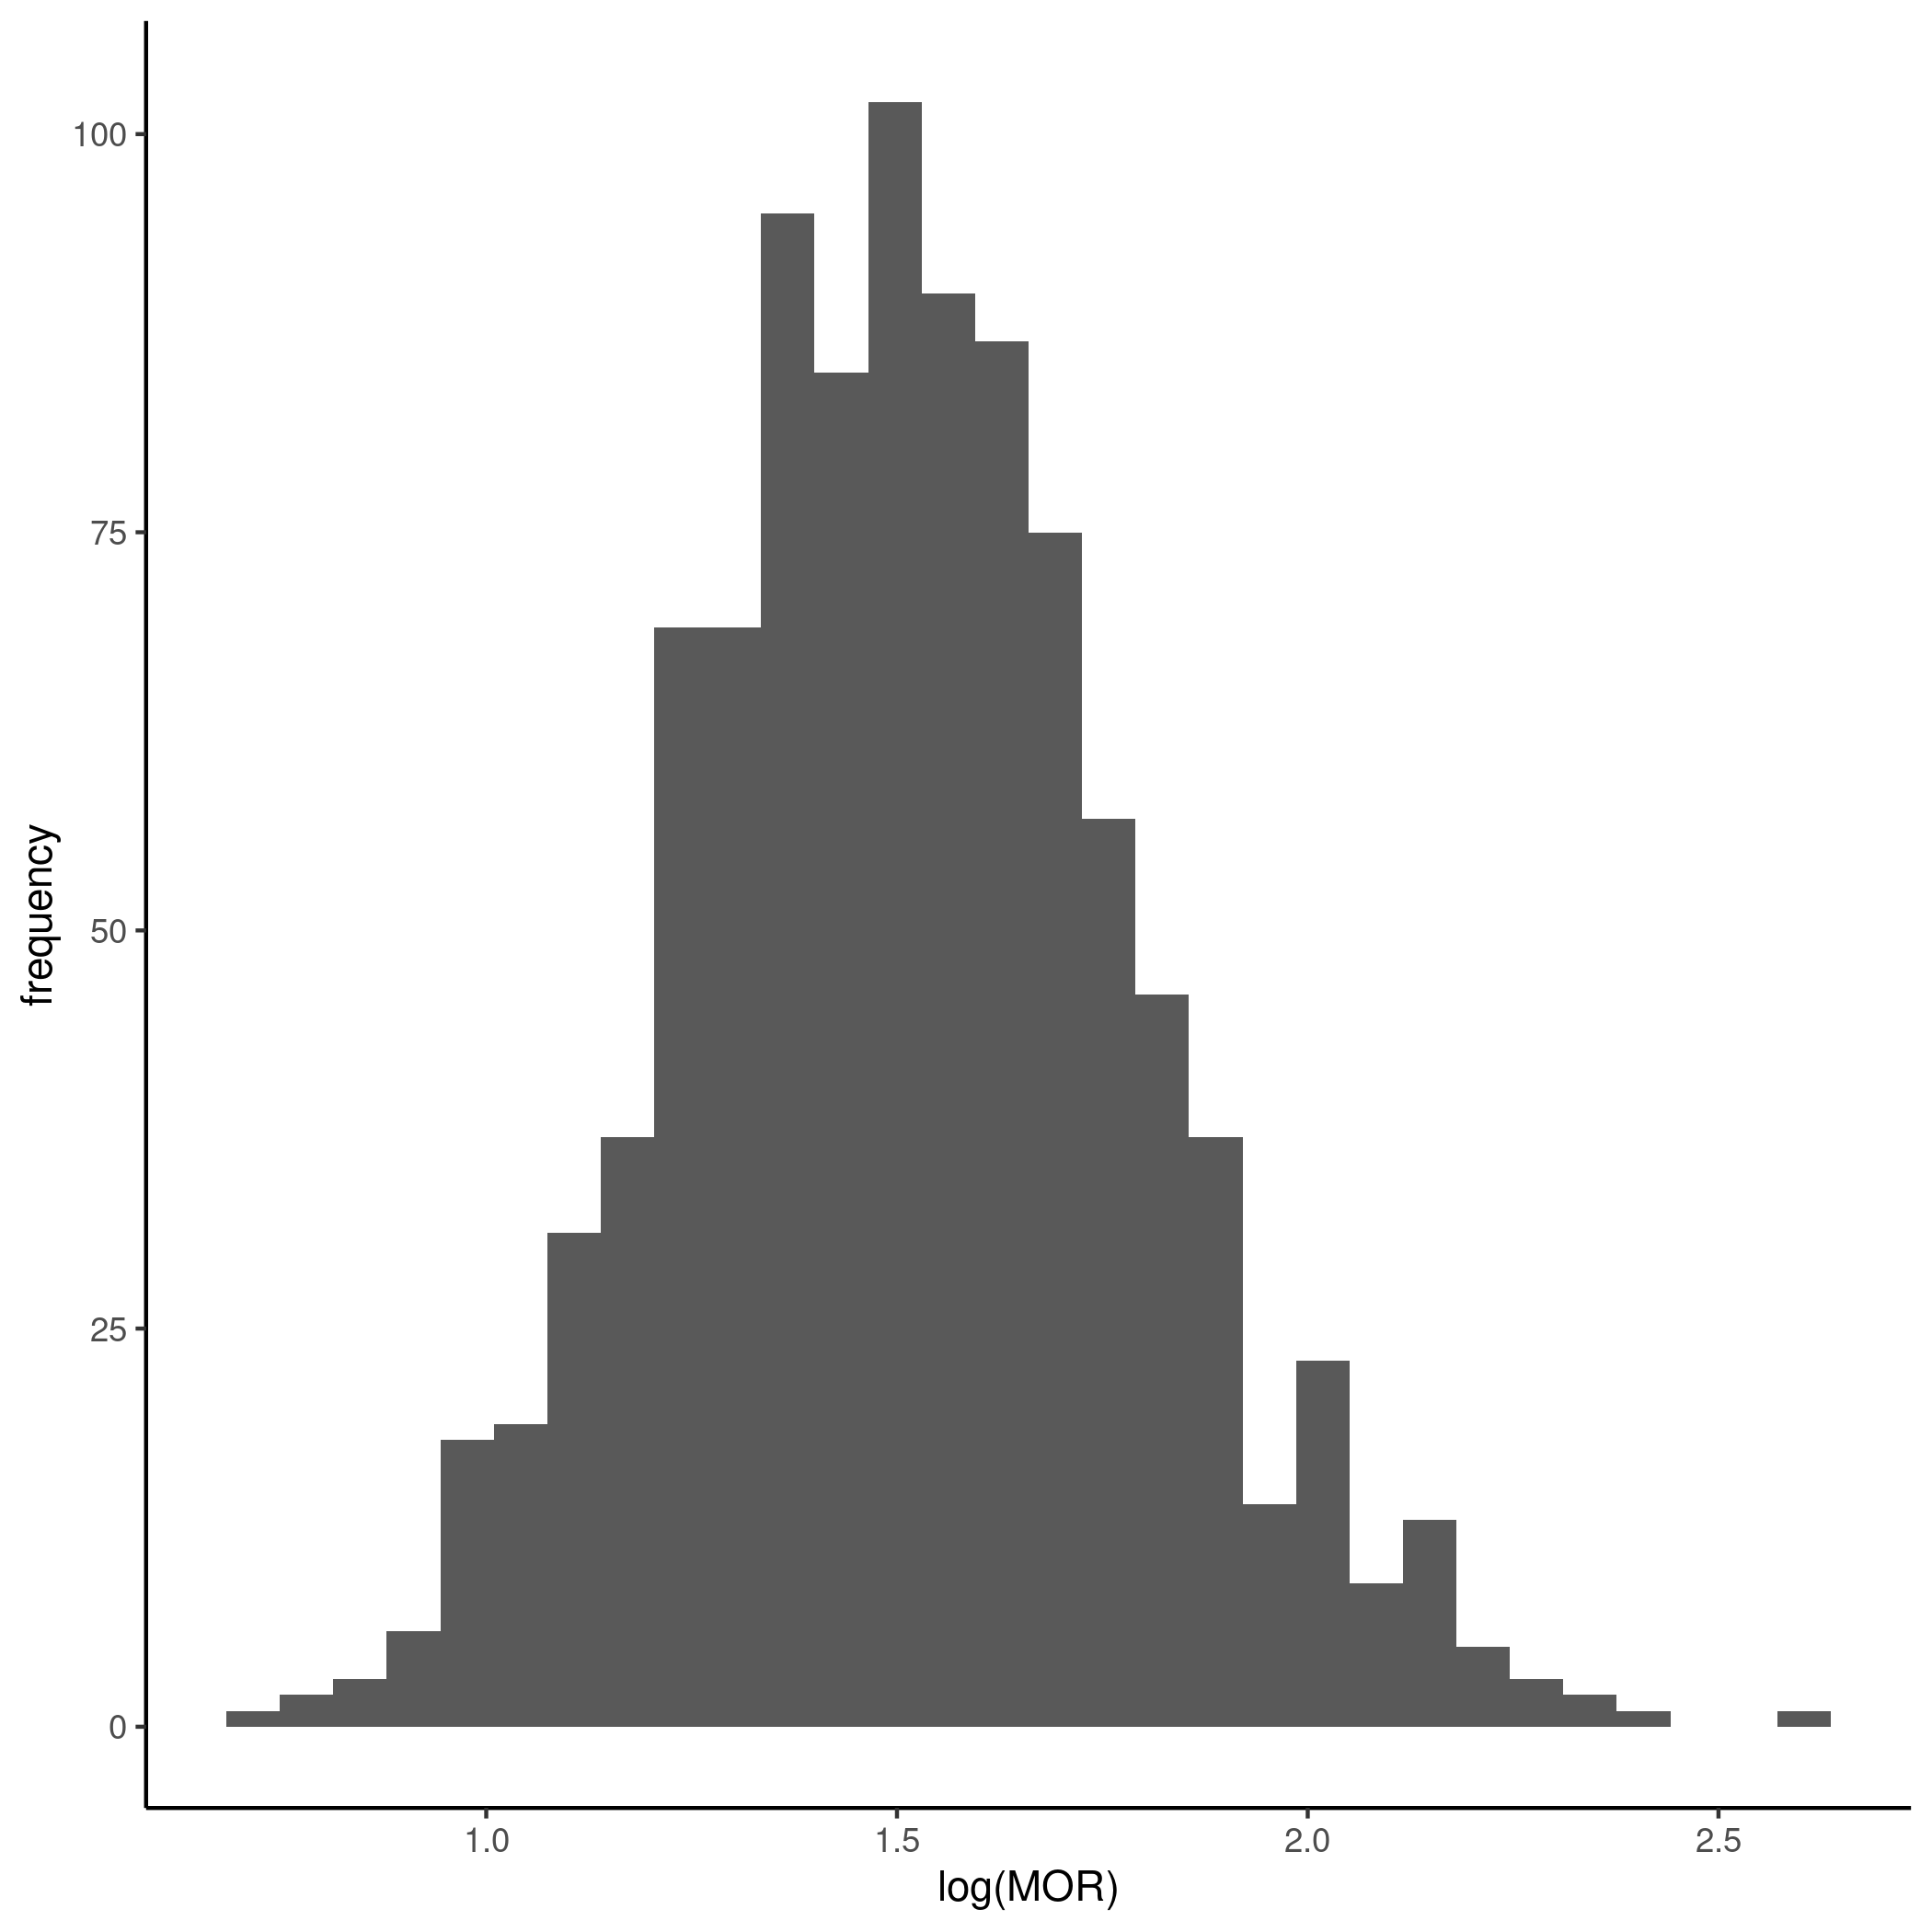
\includegraphics{../../plots/two-lvl-ran-int/high-prev/hist_100_5_two_lvl_high_prev.png}

}

\caption{Cluster size 5}

}

\end{minipage}%
%
\begin{minipage}[t]{0.24\linewidth}

{\centering 

\raisebox{-\height}{

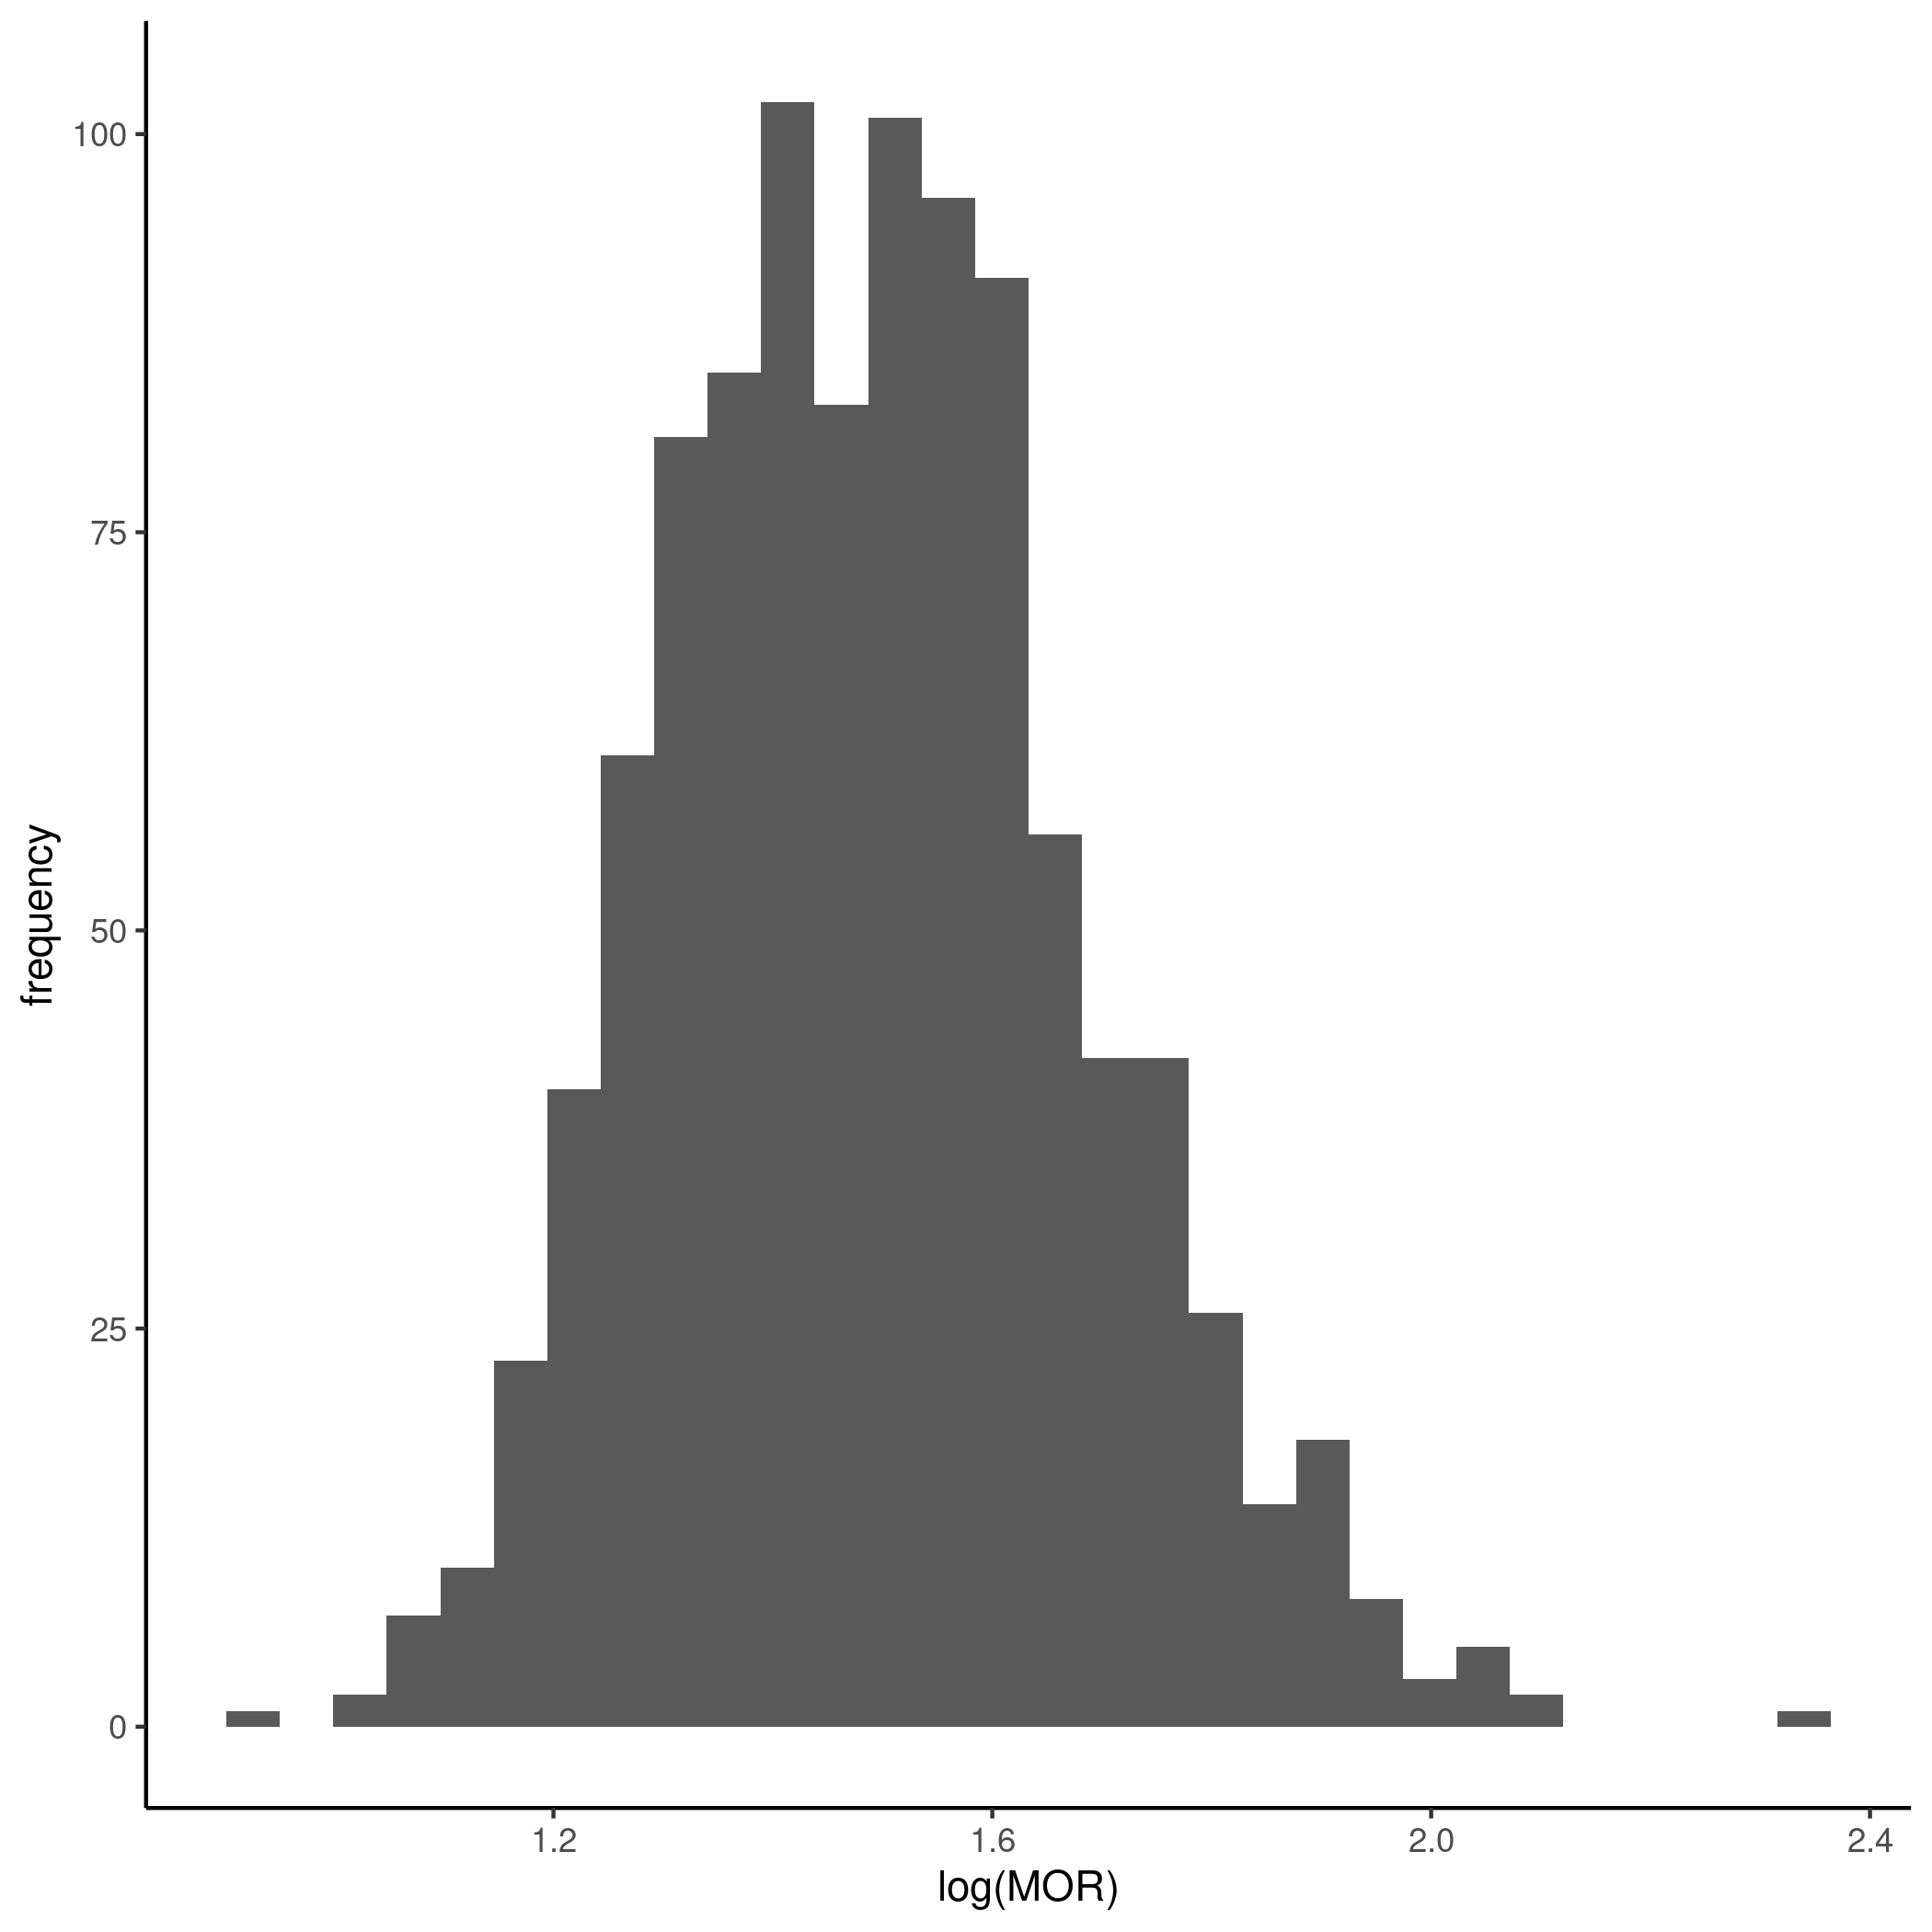
\includegraphics{../../plots/two-lvl-ran-int/high-prev/hist_100_10_two_lvl_high_prev.png}

}

\caption{Cluster size 10}

}

\end{minipage}%
%
\begin{minipage}[t]{0.24\linewidth}

{\centering 

\raisebox{-\height}{

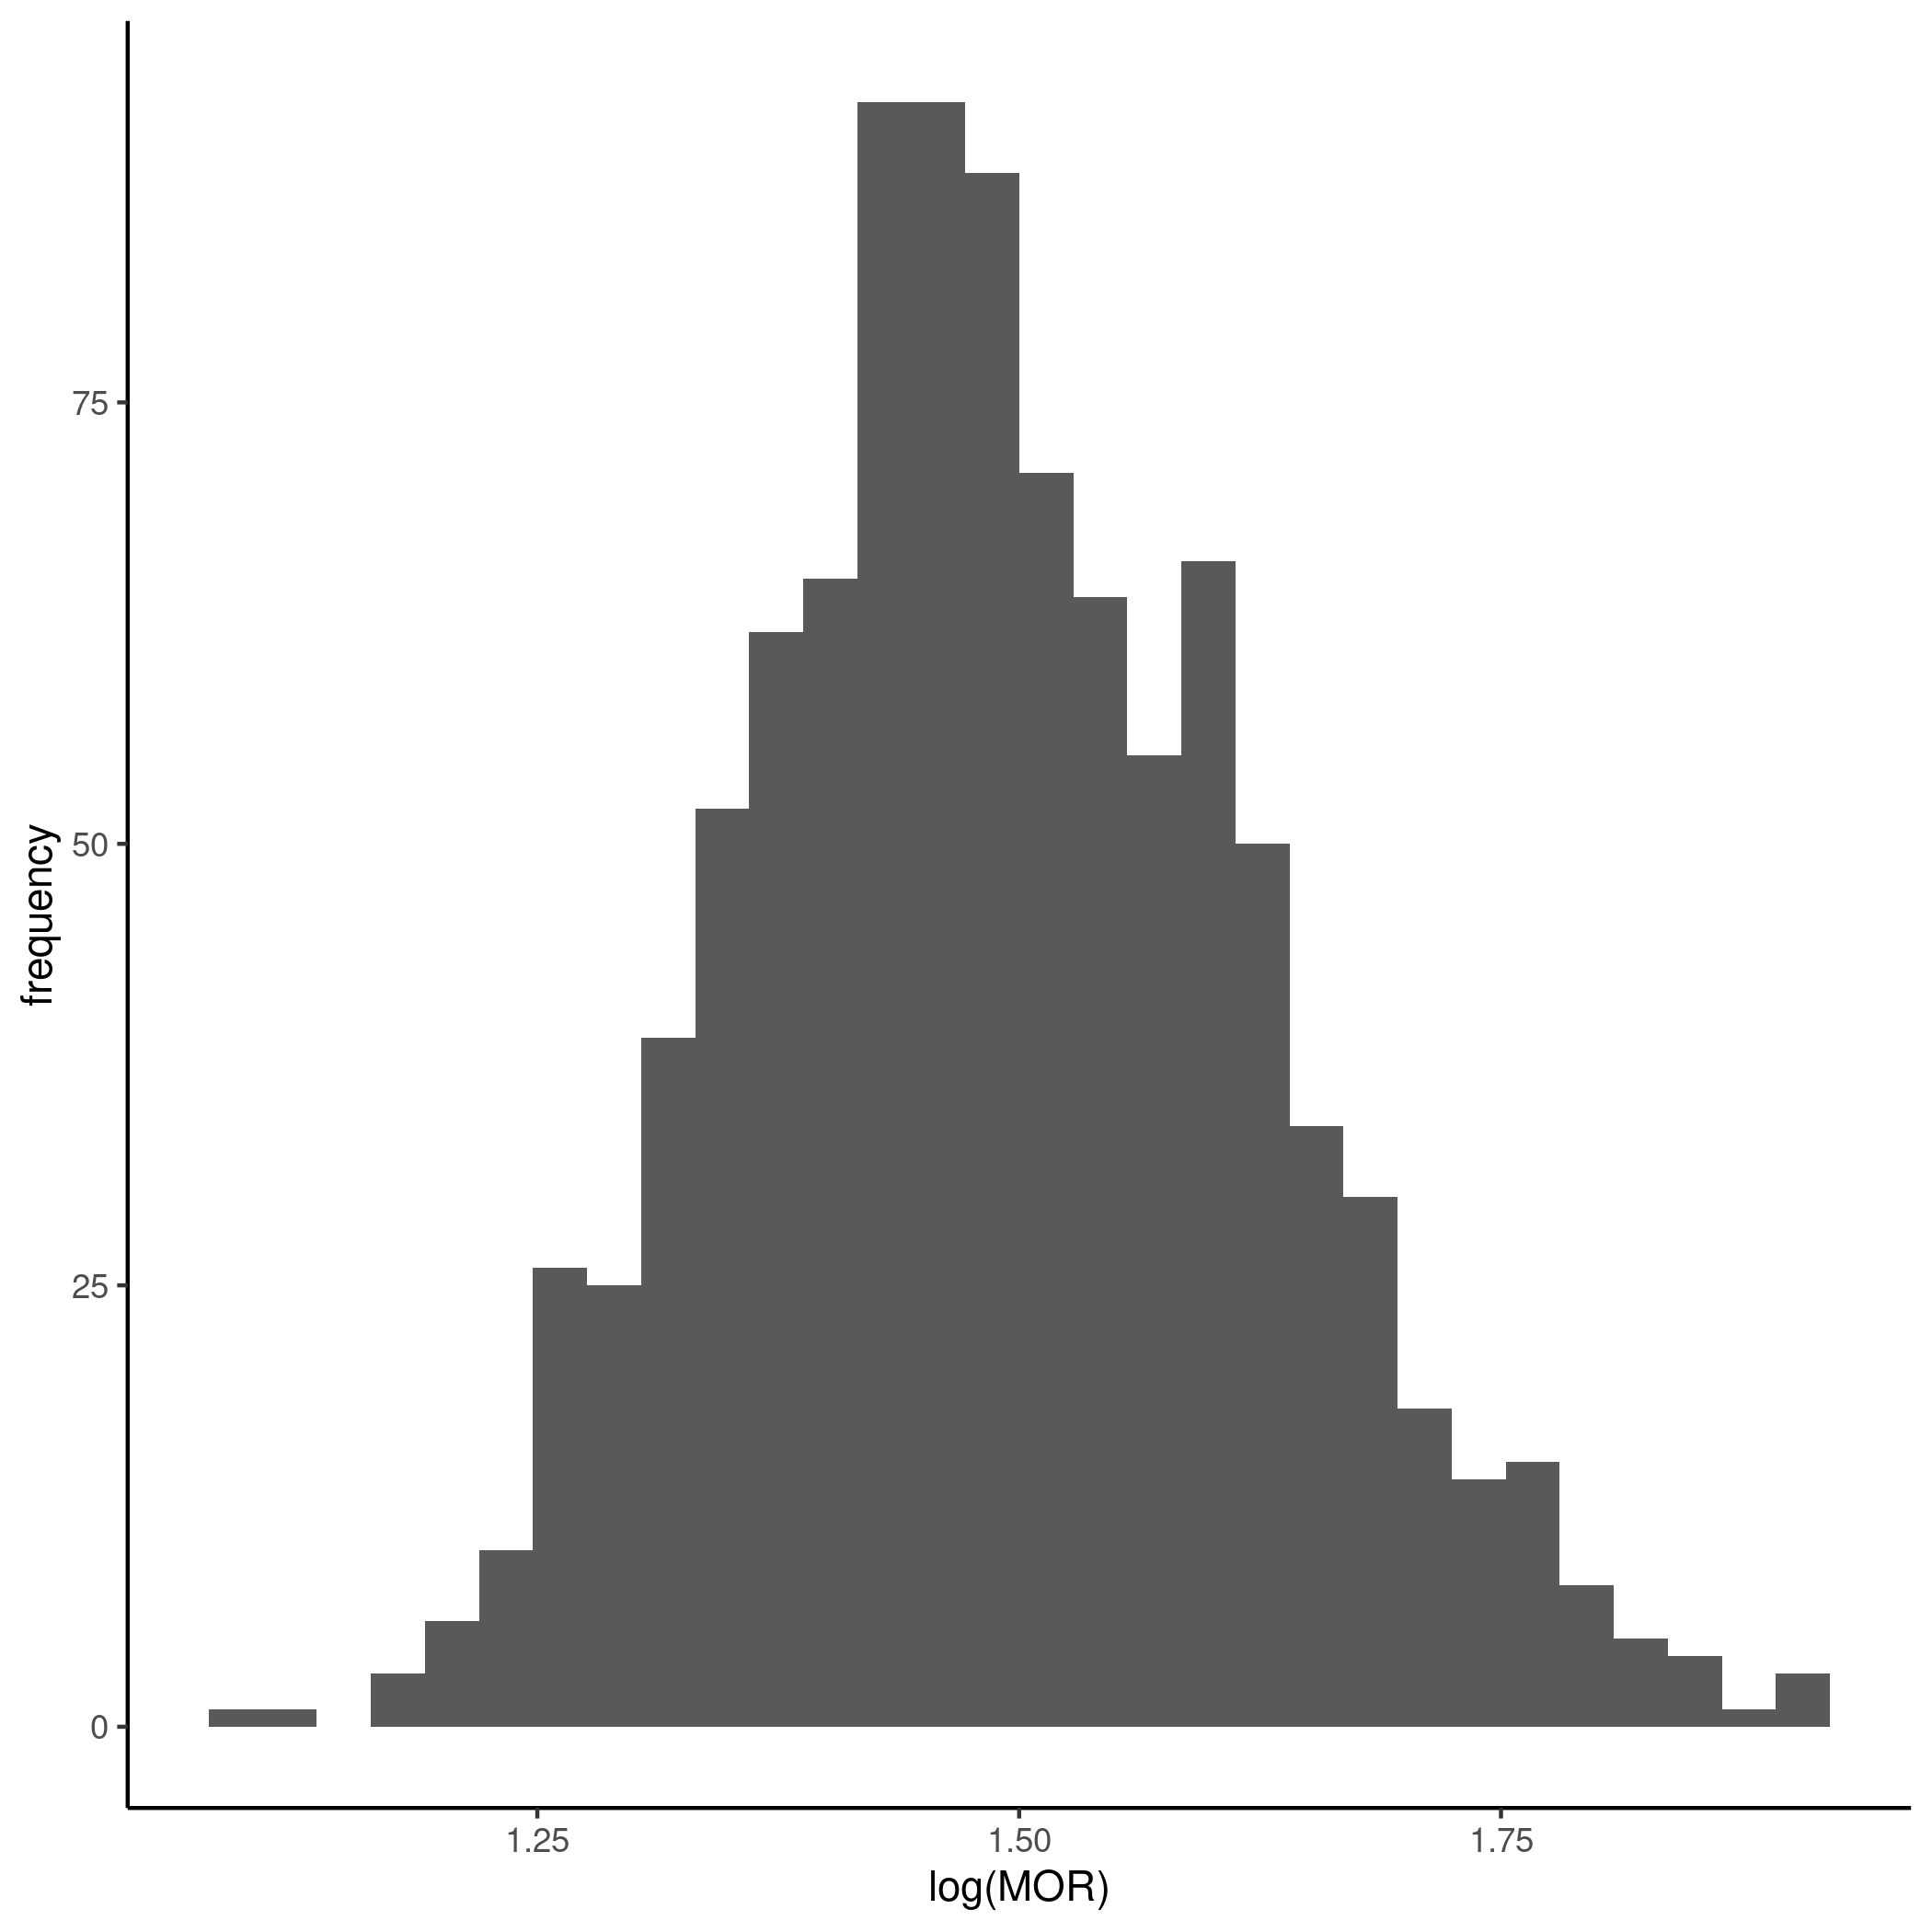
\includegraphics{../../plots/two-lvl-ran-int/high-prev/hist_100_30_two_lvl_high_prev.png}

}

\caption{Cluster size 30}

}

\end{minipage}%
%
\begin{minipage}[t]{0.24\linewidth}

{\centering 

\raisebox{-\height}{

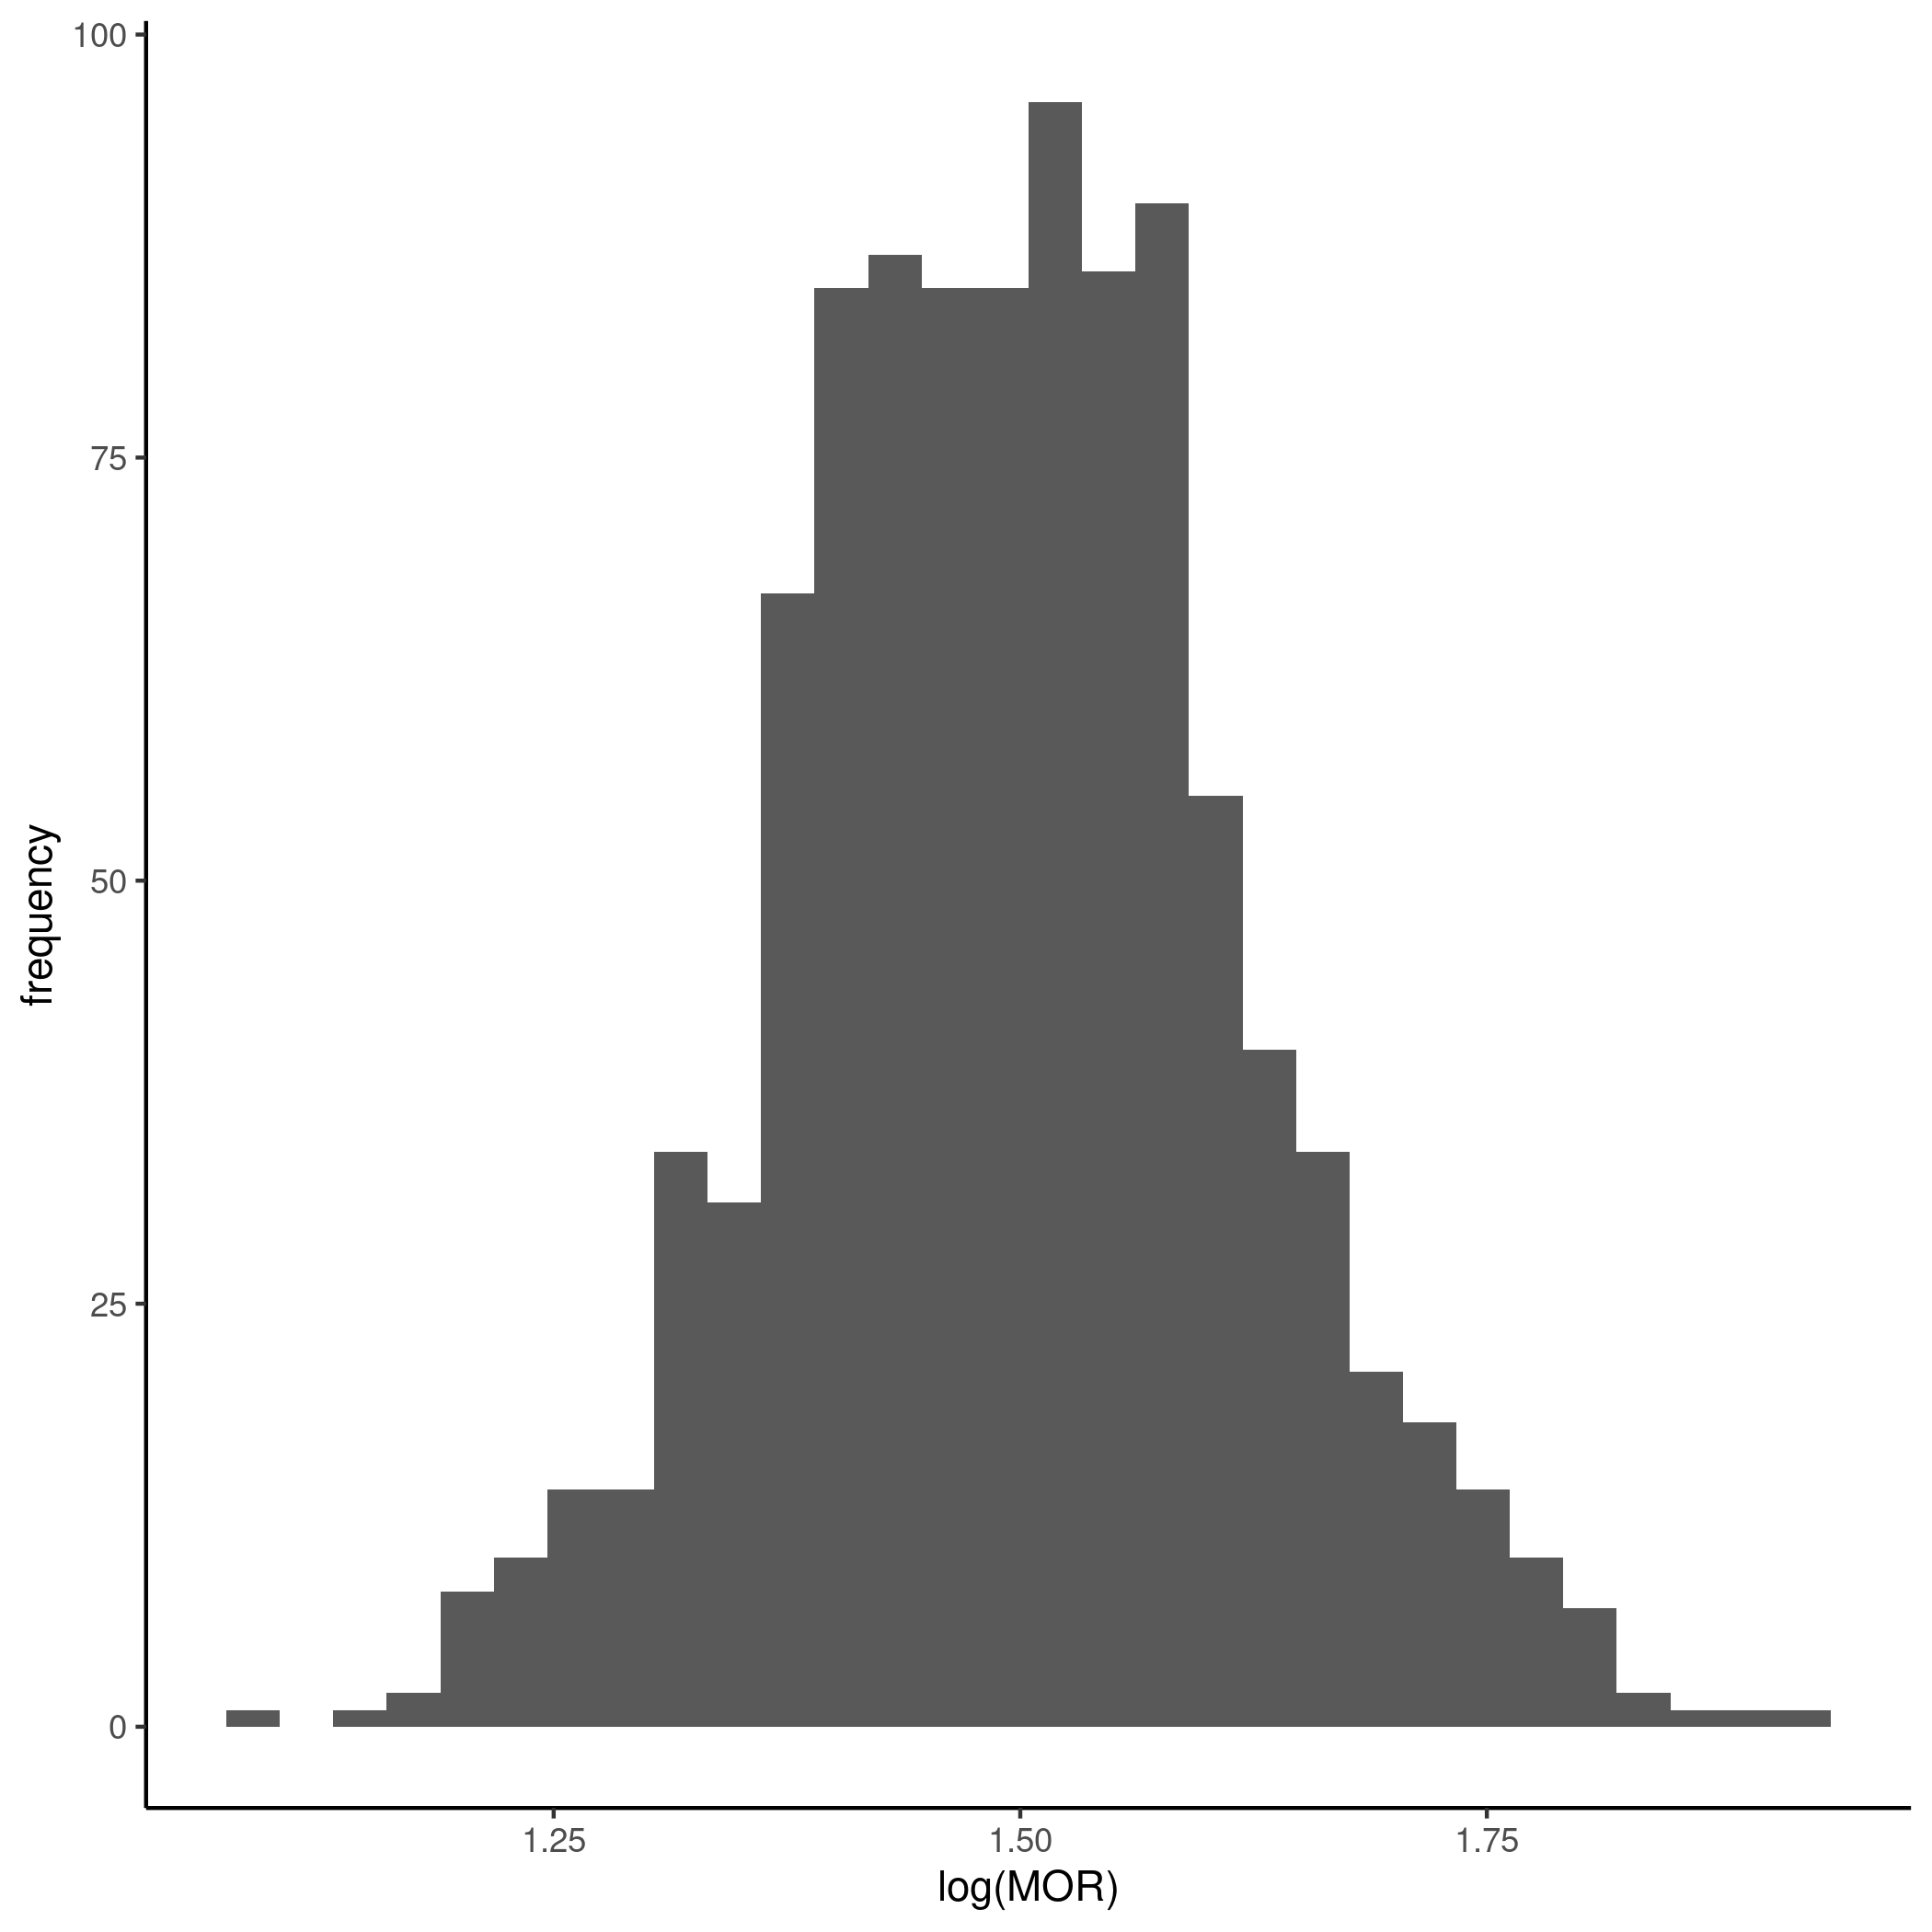
\includegraphics{../../plots/two-lvl-ran-int/high-prev/hist_100_50_two_lvl_high_prev.png}

}

\caption{Cluster size 50}

}

\end{minipage}%

\end{figure}

\newpage

\KOMAoptions{usegeometry,paper=landscape,pagesize}
\recalctypearea
\newgeometry{right=10mm,left=10mm}

\hypertarget{simulation-result-table}{%
\section{Simulation Result Table}\label{simulation-result-table}}

\begingroup

\fontsize{10pt}{14pt}\selectfont
\addtolength{\tabcolsep}{0.1pt}

\begin{tabular}[t]{>{\centering\arraybackslash}m{1.55cm}>{\centering\arraybackslash}m{1.55cm}>{\centering\arraybackslash}m{1.55cm}>{\centering\arraybackslash}m{1.55cm}>{\centering\arraybackslash}m{1.55cm}>{\centering\arraybackslash}m{1.55cm}>{\centering\arraybackslash}m{1.55cm}>{\centering\arraybackslash}m{1.55cm}>{\centering\arraybackslash}m{1.55cm}>{\centering\arraybackslash}m{1.55cm}>{\centering\arraybackslash}m{1.55cm}>{\centering\arraybackslash}m{1.55cm}>{\centering\arraybackslash}m{1.55cm}}
\toprule
Number of Cluster & Cluster Size & $\widehat{\beta_0}$ & $\widehat{\beta_1}$ & $\widehat{\beta_2}$ & $\widehat{\sigma_u^2}$ & $\widehat{MOR}$ & Relative Bias (\%) & $\widehat{SE}_{MOR}$ & Simulation $\widehat{SE}_{MOR}$ & Ratio\textsuperscript{1} & CI coverage (95\%) & Model Convergence\\
\midrule
10 & 5 & -2.05 & 2.03 & 0.70 & 3.10 & 6.41 & 41.80 & 3.07 & 2.40 & 1.28 & 0.94 & 0.88\\
10 & 10 & -1.92 & 1.88 & 0.69 & 2.82 & 5.50 & 21.65 & 1.93 & 1.88 & 1.02 & 0.94 & 0.98\\
10 & 30 & -1.90 & 1.80 & 0.68 & 2.47 & 4.67 & 3.43 & 1.53 & 1.58 & 0.97 & 0.88 & 1.00\\
10 & 50 & -1.88 & 1.78 & 0.70 & 2.30 & 4.37 & -3.36 & 1.46 & 1.49 & 0.98 & 0.86 & 1.00\\
\midrule
30 & 5 & -1.94 & 1.86 & 0.67 & 2.87 & 5.42 & 19.86 & 1.70 & 1.71 & 1.00 & 0.97 & 0.99\\
30 & 10 & -1.88 & 1.80 & 0.67 & 2.58 & 4.74 & 4.88 & 1.41 & 1.43 & 0.99 & 0.94 & 1.00\\
30 & 30 & -1.86 & 1.76 & 0.68 & 2.48 & 4.54 & 0.50 & 1.28 & 1.29 & 0.99 & 0.92 & 1.00\\
30 & 50 & -1.87 & 1.76 & 0.68 & 2.45 & 4.49 & -0.57 & 1.25 & 1.25 & 1.00 & 0.91 & 1.00\\
\midrule
50 & 5 & -1.90 & 1.82 & 0.67 & 2.76 & 5.08 & 12.48 & 1.49 & 1.52 & 0.98 & 0.96 & 1.00\\
50 & 10 & -1.89 & 1.79 & 0.68 & 2.60 & 4.72 & 4.41 & 1.31 & 1.31 & 1.00 & 0.94 & 1.00\\
50 & 30 & -1.86 & 1.76 & 0.67 & 2.48 & 4.52 & -0.04 & 1.21 & 1.21 & 1.00 & 0.93 & 1.00\\
50 & 50 & -1.87 & 1.76 & 0.67 & 2.46 & 4.48 & -0.78 & 1.19 & 1.18 & 1.00 & 0.95 & 1.00\\
\midrule
100 & 5 & -1.87 & 1.76 & 0.66 & 2.61 & 4.74 & 4.83 & 1.31 & 1.32 & 0.99 & 0.94 & 1.00\\
100 & 10 & -1.87 & 1.76 & 0.67 & 2.50 & 4.54 & 0.56 & 1.20 & 1.21 & 0.99 & 0.94 & 1.00\\
100 & 30 & -1.86 & 1.75 & 0.67 & 2.46 & 4.48 & -0.85 & 1.14 & 1.14 & 1.00 & 0.94 & 1.00\\
100 & 50 & -1.86 & 1.75 & 0.67 & 2.48 & 4.50 & -0.37 & 1.13 & 1.13 & 1.00 & 0.95 & 1.00\\
\bottomrule
\multicolumn{13}{l}{\rule{0pt}{1em}\textit{Note: }}\\
\multicolumn{13}{l}{\rule{0pt}{1em} }\\
\multicolumn{13}{l}{\rule{0pt}{1em}\textsuperscript{1} Ratio$\;=\;\dfrac{\widehat{SE}_{MOR}}{Simulation\;\widehat{SE}_{MOR}}$}\\
\multicolumn{13}{l}{\rule{0pt}{1em}\textsuperscript{*} The mean prevalence for this simulation is 29\%}\\
\multicolumn{13}{l}{\rule{0pt}{1em}\textsuperscript{\dag} True $MOR$ is 4.52}\\
\multicolumn{13}{l}{\rule{0pt}{1em}\textsuperscript{\ddag} True $\sigma^2_u$ is 2.5}\\
\multicolumn{13}{l}{\rule{0pt}{1em}\textsuperscript{\S} True Values of $\beta_0 = -1.85$, $\beta_1 = 1.75$, $\beta_2 = 0.67$}\\
\end{tabular}

\endgroup



\end{document}
